
\begin{figure}
    \centering
    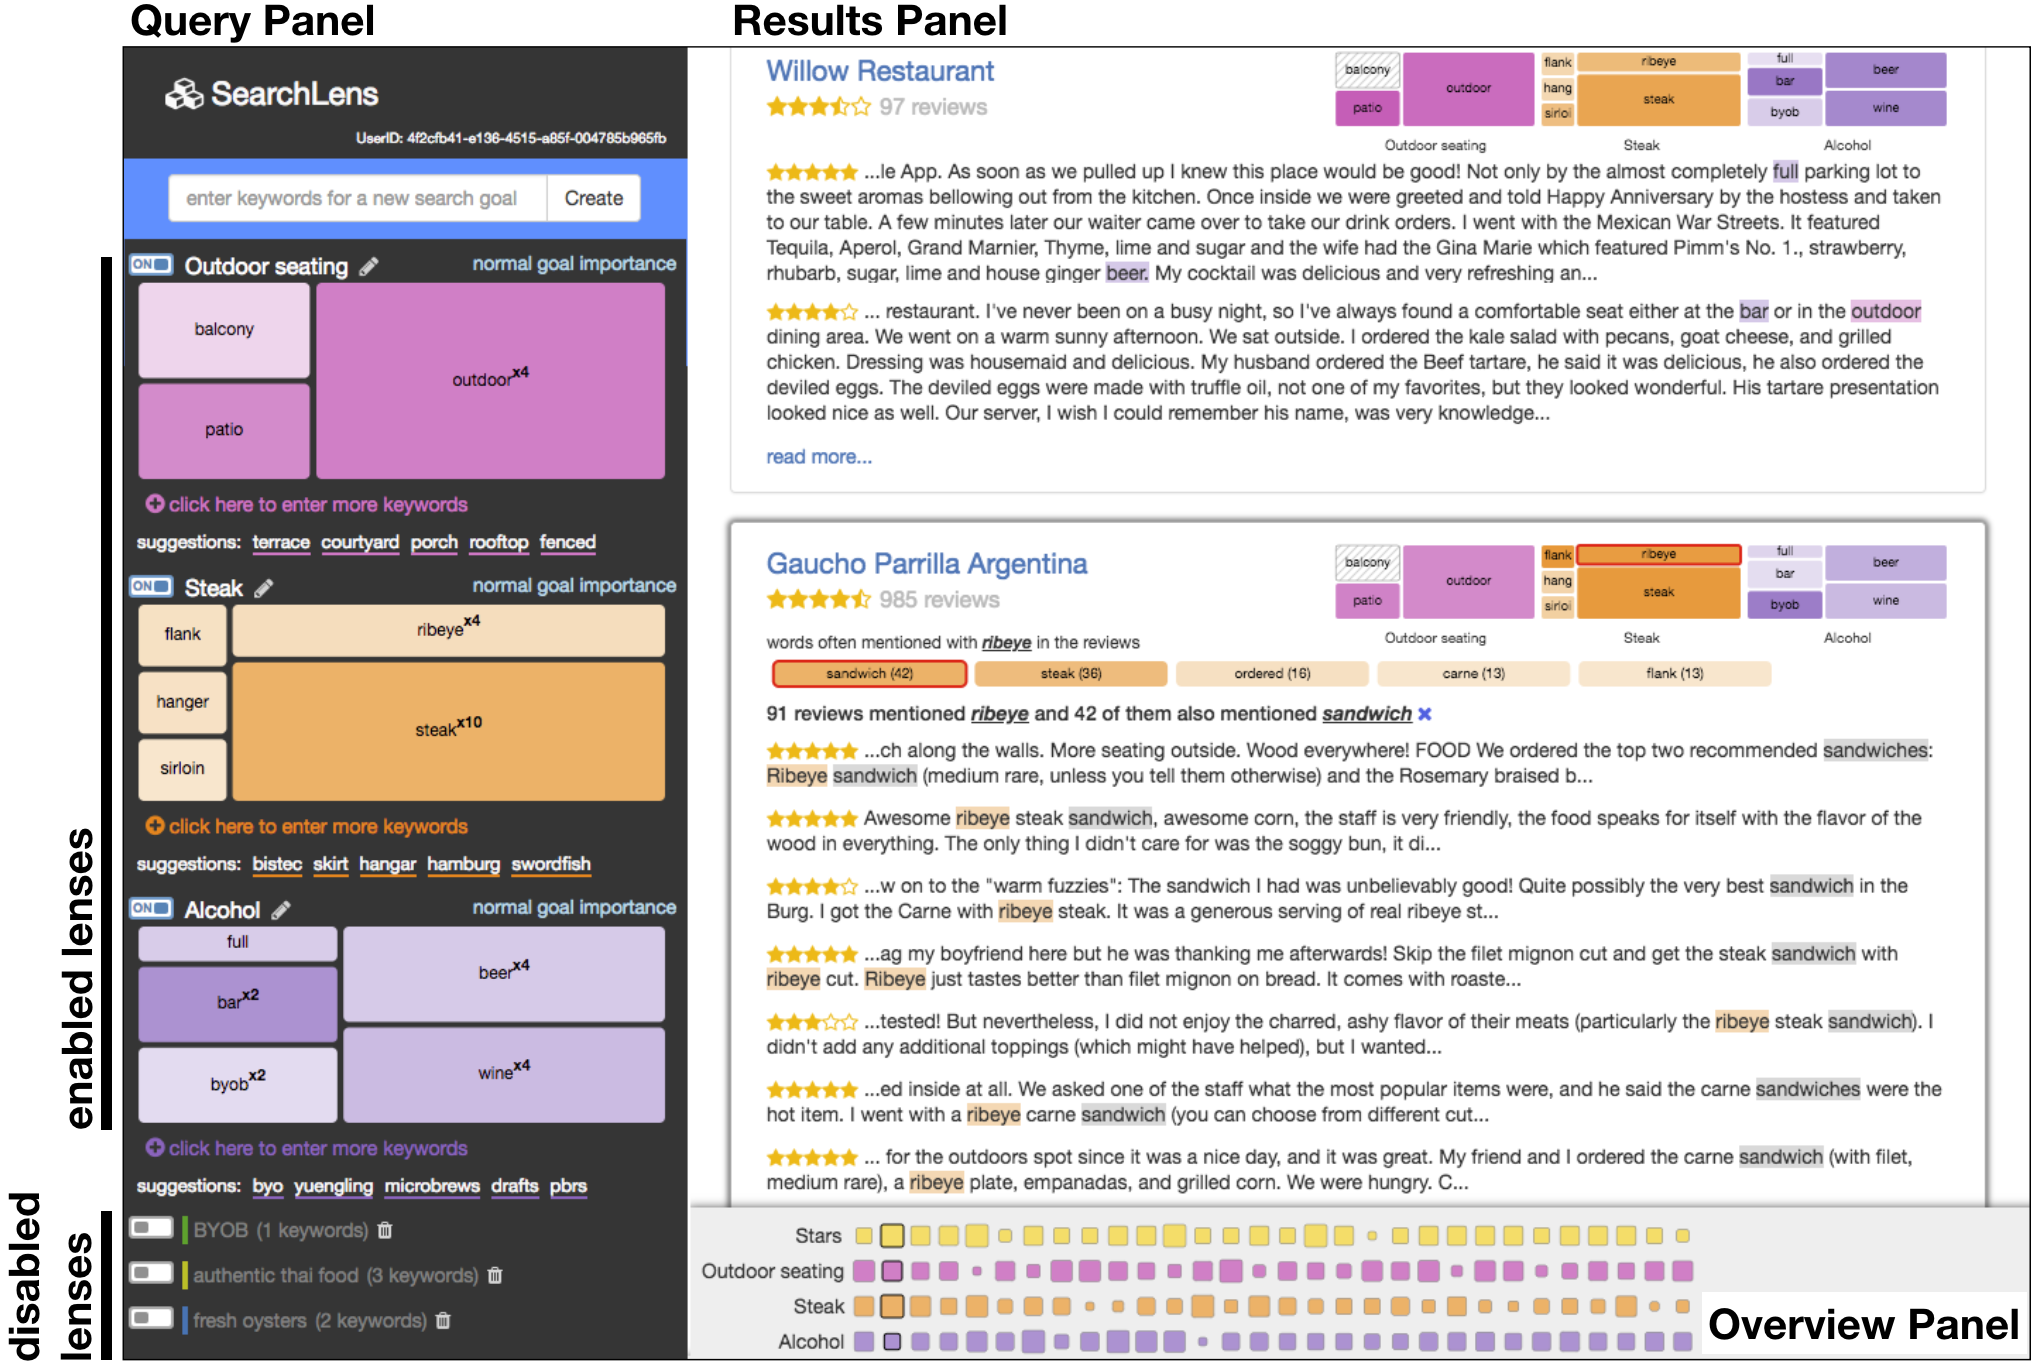
\includegraphics[width=1.0\textwidth]{Chapters/SearchLens/figures/main_annotated.png}
    \caption[An overview of the SearchLens system.]{An overview of the SearchLens system. The Query Panel on the left allows users to specify search topics, or Lenses, by specifying multiple keywords. The keywords for a given Lens are show in colored cells sized by importance (weight). Lenses can be freely disabled or enabled for different scenarios. The Results Panel on the right shows a ranked list of search results that best match the enabled Lenses from the searcher. The same visualization for specifying queries are then used for explaining how each result matches with user's interests and mental model, and also serve as an interactive navigation for filtering mentions of specific keywords. The Overview Panel at the bottom shows a collapsed version of the cells that allows for quick comparison between results.}
    \label{fig:sl_flow}
\end{figure}

\section{Introduction}

People often rely on reading online reviews and forum posts to make predictions about how well different options might match their personal interests and needs.  With the proliferation of online reviews, people now have instant access to millions of online reviews from people with varying perspectives and interests. It was estimated that in 2013 Amazon provided shoppers access to more than one million reviews for just their electronics section \cite{mcauley2013hidden}, and in 2016 Yelp provided around 250,000 reviews for over 6,000 restaurants for the city of Toronto alone \cite{yelpdata}. Having access to this rich repository of diverse perspectives based on the past experiences of others has the potential to empower consumers to understand their choices thoroughly and make better decisions for themselves without being overly influenced by marketing and branding \cite{de2015navigating}.

%However, the diversity of the reviews also often makes aggregated information, such as average review ratings, not enough for people to make decisions, and finding relevant reviews and reading through to understand the decision space can be challenging and time-consuming because people must both discover important factors that might be relevant to them (e.g., long lines, dishes or ingredients that signal the authenticity of food) as well as evaluate how various options address those factors. Furthermore, once they have finished searching the work they did in discovering factors and evaluating options does not persist, resulting in them having to start from scratch even for a very similar need. For example, a traveler who has spent a lot of time choosing between ramen restaurants in Los Angeles must start from scratch evaluating ramen restaurants in Toronto, despite having discovered several important factors (e.g., thickness and chewiness of noodle, whether the broth is simmered for a long time with pork bones) that will be similarly utilized in their decision making.

% I added this back for people who might say why not just look at the scores
Unfortunately, it is often difficult for users to be able to quickly and efficiently match their personal interests to the large amount of information available for each potential option. One problem is that simple star ratings are often not sufficient, and recent research has shown reviews often play an important role in users online purchase decisions \cite{mudambi2010research,gan2012helpfulness}. For example, restaurants might receive negative reviews for its simple decor and lack of good ambiance, but some searchers might value more the authenticity of the food or whether vegan options were available on the menu. Subsequently, finding, reading, and evaluating relevant reviews is time-consuming and challenging. Users have to manually parse through the reviews for each restaurant and match them to their personal interests (e.g., kid friendly, authentic Indian cuisine). They then have to track which restaurant meets which criteria, and if they discover and add any additional criteria, they must back-fill that information and re-evaluate previously seen restaurants. Furthermore, once a user has finished searching, the work performed discovering and evaluating factors is lost, resulting in having to start from scratch even if a similar need arises in the future. For example, a traveler who has spent a lot of time choosing between ramen restaurants in Los Angeles must start from scratch evaluating ramen restaurants in Toronto, despite having discovered several important factors (e.g., thickness and chewiness of noodle, whether the broth is simmered for a long time with pork bones) that will be similarly utilized in their decision making.

Getting users to specify these nuanced interests and preferences has been a long standing challenge. Several decades of research have explored ways of getting users to externalize their interests \cite{jansen2000real,belkin2001rutgers}, for example by: using prompt and text field designs that promote longer query terms \cite{franzen2000verbosity,belkin2003query}, asking for relevance feedback on the results provided \cite{salton1990improving,rui1998relevance,peltonen2017negative}, or explicitly asking users to build up sets of query terms of different topics \cite{hearst1996visualizing,hoeber2006comparative}. There are two primary challenges brought up by this work. First, users have trouble specifying their interests, which includes challenges with identifying query terms that were neither too general nor too specific; providing more than a few terms (even when longer queries were more likely to lead to useful results); and learning terms from the content, rather than knowing them all beforehand  \cite{belkin2003query,salton1990improving}. The other main issue found is that it is very difficult to get users to put in the work to externalize their interests, either as query terms or as explicit feedback, due to perceptions that the work will not be sufficiently paid off in the future or not understanding how their work will affect their results. 
%% This is unnecessary and very repetitive with the previous paragraph

To tackle this issue of capturing, leveraging and exposing user interests, we introduce SearchLense, where users construct externalized representations of their interests as ``Lenses''. Lenses are leveraged as an explanatory tool, providing users with a way to quickly parse, understand and make judgments based on the vast amount of review data instantaneously. Additionally, Lenses can be reused in different contexts and combined in different configurations. In the example above, imagine a system which could capture the factors that the traveler found important for ramen in Los Angeles and reuse them to quickly make a confident, personalized decision about ramen in Toronto. If traveling to Toronto with kids, a ``kids'' Lens might also be added with factors such as whether the restaurant typically has long lines and how many seats it has. These persistent Lenses could be useful in a variety of situations beyond reviews, ranging from academics keeping track of interesting research topics; travelers deciding which places to visit in an unfamiliar city; consumers deciding between products; lawyers doing case discovery; or voters tracking important issues.
We explore this problem in the context of restaurant reviews, conducting a controlled lab study with 29 participants to examine if our visual interface for explanation and exploration is effective in providing immediate benefits to elicit rich interest expressions from the users. Additionally, we performed a three day field deployment study with 5 participants to explore the benefits of Lenses when users were conducting their own tasks. Results suggest that our prototype system SearchLens was able to learn richer representations of its users' interests when compared to a baseline system by allowing users to fluidly capture, build, and refine Lenses to reflect their interests and needs, and that the user-generated interfaces can be reused over time and transfer across contexts.


%% See Comment
%To understand the prevalence of these issues, we conducted a pilot survey with 50 participants recruited from Amazon Mechanical Turk (age between 21 and 63, M=37.0, SD=11.7, 52\% male, and 48\% female, mostly from the US), focusing on their experiences when researching restaurants online. We chose restaurant search as our main topic due to its subjective nature and the availability of large repositories of reviews with diverse opinions and preferences. Most of our participants (95\%) self-reported that they use services that provide reviews and ratings to look for restaurant information online. At the same time, 60\% of the participants agreed that do not always choose restaurants based on their average ratings. Participants also agreed that when searching for restaurants online, they had encountered restaurants with bad average ratings but were mostly about things that they did not care about (62\%), and that it is time consuming to sift through reviews to find ones that were of interest to them (60\%). This suggests that searchers often spend a lot of time and effort to carefully examine the reviews and identify relevant aspects and keywords that reflect their personal preferences and repeat this process across different scenarios.



% MERGED INTO (2) -- ; and 3) users do not understand how their interactions will affect their content. 
% i feel like (2) and (3) is potentially saying how the interaction of querying is agent-based since the relationship between input and output is unclear and can be unexpected, and we are making it towards direct manipulation by adding transparency 

%Supporting personalized explanation of items in a search results is challenging first because the interests and goals of an individual are often not fully specified in the query, and then were often further compressed by computational representations that can be difficult for humans to understand \cite{chuang2012interpretation}. 
%Consider for example an user interested in authentic Indian food -- this may be true at a high level, but perhaps that person also has a preference towards Northern Indian cuisine, and has particular specific favorites, such as \textit{pani puri} or \textit{samosas}. Or perhaps users are trying to look for \textit{outdoor restaurants} in a \textit{easy-to-park neighborhood} that have \textit{space for kids} to run around but also serve \textit{hoppy beers} and \textit{rye whiskey}. If these nuanced interests and soft criteria, while often key factors in decision making, are  not specified in the query terms, search systems would have little understanding of their users to generate personalized explanation for each result, leaving users to rely on closely examining many reviews to identify ones that were relevant to their latent interests in order to comprehend options in the search results.



% Results suggest that our prototype system SearchLens can:

% \begin{itemize}
% \item allow users to fluidly capture, compose, and reuse Lenses to reflect their interests and needs for different contexts
% \item allow users to interpret, explore, and discover desired results using personalized interactive interfaces instead of sifting through reviews in arbitrary order
% \item encourage users to express and refine their Lenses using significantly more keywords when compared to a baseline condition that does not support personalized explanation and exploration interfaces
% \end{itemize}

%However, the sheer amount of online reviews are often well beyond individuals capacity to process, prohibiting them to benefit fully from the these rich repositories of diverse information.
%While review services typically provide users with average rating score and rating distribution for each option, they provide little personalized insights into how each option matches with the interests of a particular user.  Supporting personalized explanation of items in a search results is challenging first because the interests and goals of an individual are often not fully specified in the query, and then were often further compressed by computational representations that can be difficult for humans to understand \cite{chuang2012interpretation}. Consider for example an user interested in authentic Indian food -- this may be true at a high level, but perhaps that person also has a preference towards Northern Indian cuisine, and has particular specific favorites, such as \textit{pani puri} or \textit{samosas}. Or perhaps users are trying to look for \textit{outdoor restaurants} in a \textit{easy-to-park neighborhood} that have \textit{space for kids} to run around but also serve \textit{hoppy beers} and \textit{rye bourbon}. Past work have shown that even expert searchers typically do not use more than a few query terms to specify their information needs, even when longer queries tend to lead to better results or higher user satisfaction in exploratory search scenarios \cite{belkin2003query}. As a result, these nuance interests and soft criteria, while often key factors in decision making, are rarely specified in a single query. This leaves search systems with little understanding of their users to generate personalized explanation for each result, leaving users to rely on closely examining many reviews to identify ones that were relevant to their latent interests in order to comprehend options in the search results.

% To understand the prevalence of this issue, we conducted a pilot survey with 50 participants recruited from Amazon Mechanical Turk (age between 21 and 63, M=37.0, SD=11.7, 52\% male, and 48\% female, mostly from the US), focusing on their experiences when researching restaurants online. We chose restaurant search as our main topic due to its subjective natural and the availability of large repositories of reviews with diverse opinions and preferences. Most of our participants (95\%) self-reported that they use services that provide reviews and ratings to look for restaurant information online. At the same time, 60\% of the participants agreed that restaurants they like do not always have high average ratings. Participants also agreed that when searching for restaurants online, they had encountered restaurants with bad average ratings but were mostly about things that they did not care about (62\%), and that it is time consuming to sift through reviews to find ones that were of interest to them (60\%). This suggests that even though modern search engines can return a list of options and reviews in split seconds, searchers often still need to spend a lot of time and effort carefully examining each result to find parts that are relevant to them before they can start comparing their options and make decisions.
% For example, looking for reviews that describe a particular drink, or whether the environment was kid friendly.

%An alternative approach is to annotation each item in the dataset of with different criteria, subtopics, and attributes, whether using expert labelers or computational techniques \cite{}, and present these metadata to the users using faceted search interfaces \cite{hearst2006design}.
%While expert annotation have found to be useful for providing an overview of a large number of choices (e.g., products, restaurants), allowing users filter and navigate to different options based on objective criteria (e.g., price range, location), it is unlikely for it to scale and support the above mentioned subjective interests and needs (e.g., good date night restaurants). For this, prior work has also explore ways to extract aspects and subjective judgments from the reviews using computational approaches. However, 

%In summary, we suggest to design exploratory search interfaces that can provide personalized explanations and exploration interfaces for each search result, and encourage users to express their rich latent interests in order to enable these benefits. In addition, many preferences (such as \textit{hoppy beers} and \textit{rye bourbon}) might be relevant for multiple contexts, such as on a date night or going out for drinks with friends in different neighborhoods, and allowing users to structure and persist keywords that describe their different interests can further reduce future efforts. This also has the benefit of encouraging users to refine their query terms to be used again in the future, since some of the terms that might seem to be good at first might in fact not be very discriminatory (e.g., \textit{great}, \textit{delicious}) versus less obvious terms that act as more ``honest signals'' (e.g., the use of the word \textit{bone broth} for ramen broth that is simmered for days).  

% In this paper we explore a novel interface that allows users to specify and maintain their multifarious and idiosyncratic search goals with structured queries that we call Lenses, and gradually construct an personalized interactive search interface based on their own interests and past activities. With the rich interest profiles specified by the users, the system can provide personalized visual explanation of items in a search results beyond average ]rating scores. The visual explanations also serve as personalized interfaces that allow users to surface reviews that matches their different latent interests for deeper  xploration. The instantiation of this approach is a prototype system called SearchLens, which allows users to progressively and persistently build up a repository of ``Lenses'' that can be used to reflect their latent topics of interests and mental model. Users construct Lenses by specifying keywords and weights, and the system visualizes the importance and frequency of each keyword in the results for comparison. Besides specifying keywords from prior knowledge, SearchLens also provides a mechanism for users to discover and collect keywords as they look at the search results. In addition, the system provides suggested keywords for each Lens using a semantic word vector model. The Lenses that users create persist across sessions, allowing users to freely enable and disable different sets of Lenses for different occasions. For example, enabling their Lenses for ``kids friendly'', ``easy parking'', and ``home cooking'' to explore restaurant options for a big family dinner, and enabling their Lenses for ``cozy and intimate'', ``easy parking'', and ``good wine selection'' to explore restaurant options for date night. These Lenses in turn allow the system to present each result based on the current interests of the users, and allow them to explore each of the results by revealing mentions of different query terms. We conducted a lab study with 29 participants, and a field study with 5 participants conducting their own tasks over 3 days. 
%In addition, we also show that standard information retrieval systems (i.e., document search engines) can be easily adapted to support these interactions with high efficiency and scale. 


% In this paper we explore a novel interface that allows users to specify and maintain their multifarious and idiosyncratic search goals with structured queries that we call Lenses, and gradually construct an interactive search interface based on their own interests and past activities. The instantiation of this approach is a prototype system called SearchLens, which allows users to progressively and persistently build up a repository of ``Lenses'' that can be used to reflect their topics of interests and mental model. Users construct Lenses by specifying keywords and weights, and the system visualizes the importance and frequency of each keyword in the results for comparison. Besides specifying keywords from prior knowledge, SearchLens also provides a mechanism for users to discover and collect keywords as they look at the search results. In addition, the system provides suggested keywords for each Lens using a semantic word vector model. The Lenses that users create persist across sessions, allowing users to freely enable and disable different sets of Lenses for different occasions. For example, enabling their Lenses for ``kids friendly'', ``easy parking'', and ``home cooking'' to explore restaurant options for a big family dinner, and enabling their Lenses for ``cozy and intimate'', ``easy parking'', and ``good wine selection'' to explore restaurant options for date night. These Lenses in turn allow the system to present each result based on the current interests of the users, and allow them to explore each of the results by revealing mentions of different query terms. We conducted a lab study with 29 participants, and a field study with 5 participants conducting their own tasks over 3 days. Results show that our prototype system SearchLens a) allows users to fluidly capture, build, and refine Lenses to reflect their interests and needs, b) allows users to interpret, explore, and discover desired results using the interactive interfaces, and c) that the user-generated interfaces can be reused over time and transfer across contexts. In addition, we also show that standard information retrieval systems (i.e., document search engines) can be easily adapted to support these interactions with high efficiency and scale. 


\section{Related Work}

%In this work, we propose to support users to fluidly express and curate their different interests and criteria using ``Lenses'', and allow them to freely compose, and reuse their previously specified interests across different contexts. One key challenge is to provide immediate and sufficient benefits to the users in order to elicit their rich interests. For this, we propose to not only use users' Lenses as a way to retrieve rel event items, but also to provide visual explanations for each item and enable deeper exploration. 

Past research has proposed a variety of approaches to collecting, modeling and leveraging users' interests and intents through both interface design and computation. Our work builds on this diverse of literature by allowing the system to learn the personal interests of the users through interaction to retrieve relevant data, and present data based on its understanding of the different users. This allows us to elicit structures that can be reused across different contexts and tasks and are more nuanced and personalized to each users when compared to traditional search structures such as search results clustering or pre-compiled facets.

% Unlike simple and objective information seeking scenarios, such as finding the address of a restaurant or checking the weather, in review search scenarios, different searchers typically have varying interests and criteria, but at the same time, the reviews themselves are often also multifarious and subjective in nature and therefore do not always match the interests of every searcher \cite{mar2006exp,de2015navigating,mudambi2010research,gan2012helpfulness}. As a results, a searcher might needs to sift through many reviews to find ones that are relevant, or come up with a set of discriminative keywords for each of his or her different interests or criteria.

% Despite their ubiquity, operations for searching with multiple topics of interest as described above are poorly supported by modern approaches. Search engines have optimized for providing information as quickly as possible \cite{teevan2013slow}, such as knowledge cards in which an answer is surfaced directly on a search results page or visual carousels of possible options that a user can quickly click through \cite{yi2009discovering,bota2016playing}. These approaches excel at finding answers to objective, factual questions, but notably fail to address activities involved in complex, personalized search tasks, such as specifying multiple goals and criteria, explaining search results based on personal interests, and allowing for deeper exploration of different options for comparison \cite{marchionini2006exploratory,white2006supporting,white2009exploratory}.

% As a result, the search result list can become increasingly difficult to interpret as the user adds more keywords to their query, raising questions like how different keywords influenced the ranking, and whether each result matches with their different topics of interests. Further, in order to explore deeper to get a better understanding of their options, users would need to leave the search result list page and visit each result independently and manually extract parts that are relevant to their goals, often with the in-page keyword matching provided by the browser. 

\subsection{Eliciting and Modeling Interests and Intents}

A significant topic of research has been interfaces that can collect, explicitly or implicitly, the personal goals and interests of users as they search for information and modify their viewing of content correspondingly. While there is extensive literature on doing so in the context of personalized search and re-ranking of search results (e.g., \cite{speretta2005personalized,shen2005implicit,burges2005learning,cao2007learning}), we focus here on work that enables more interactivity and transparency of users' interests to support more complex searching.  One such thread lies in the collection of users' interests through keywords or interest vectors into an agent or user interest or intent model. This includes seminal work such as WebMate \cite{chen1998webmate}, which built up an agent composed of sets of TF-IDF \cite{wu2008interpreting} vectors to represent the user's different interests. Similar to WebMate, we aim to build collections of terms that represent the user's interests, but focus on explicit user selection of those sets, and making them explainable and composable. Interestingly, WebMate's ``Trigger Pair Model'' which looked at co-occurrence of words within a sliding window across a set of documents can be seen as a precursor to the word vector model that we use for keyword suggestions.  More recent work in this vein includes user modeling of concepts, such as AdaptiveVIBE \cite{ahn2009adaptive} and Intent Radar \cite{peltonen2017negative}, which include two dimensional visualizations of documents and their relation to the user's inferred interests. Our work builds upon these but aims at increasing the richness of the structure, nuance, and specificity of the user's expression of interests. Specifically, our Lenses, composed of multiple keywords that can capture multiple levels of specificity, can be themselves composed into more complex expressions and reused across different contexts and tasks. We also focus on supporting users in the discovery process of building good terms that are discriminatory and explanatory.


%\subsection{Exploratory Search Interfaces}

%A major thread of work that we draw on includes novel personalized search interfaces such as semantic web interfaces \cite{wilson2006mspace}, or computational approaches such as automatic or interactive result clustering \cite{cutting2017scatter}. Several exploratory search interfaces have been developed in order to help searchers orient themselves in the information space, review and explore the different subtopics, and keep track of their overall progress \cite{hearst2009search,marchionini2000agileviews,patterson2001predicting,tretter2013searchpanel,morris2008searchbar}. Two closely related studies include Topic-Relevance Map and Exploration Wall, which explored ways to provide overviews of search results of academic papers using document keywords and entities and easily choose keywords to build up subsequent queries \cite{peltonen2017topic,klouche2015designing}. In SearchLens, instead of proposing subsequent queries to the users, we instead propose potentially useful keywords to be incorporated into users' existing Lenses, and provides visual explanations for each item that are capable of scaling to many query terms. This allows users to query with many query terms instead of switching between different more focused query, while still being able to easily comprehend how each result matches with their different latent interests.

% https://www.researchgate.net/publication/221300933_An_Aspectual_Interface_for_Supporting_Complex_Search_Tasks



\subsection{Concept Discovery and Evolution}

Research in interactive machine learning has also explored techniques to support data annotators or searchers in discovering and externalizing useful concepts when working in unfamiliar domains. 
%Another line of research in interactive machine learning explored using visualization and interaction techniques to better support discovering, externalizing, and refining useful concepts while exploring and labeling data in unfamiliar domains.
For example, Alloy used a \emph{sample-and-search} technique to categorize textual datasets with novice crowdworkers where they first explore the space of information through sampling items in the dataset to discover useful categories, then externalize each category using a set of query terms and search for other relevant items \cite{alloy}.
Past work has further suggested that the working concepts of an annotator may change over time as new items were examined \cite{kulesza2014structured}. Different techniques that can better support this concept evolution process were proposed, such as structured labeling \cite{kulesza2014structured}, crowd collaboration \cite{Chang:2017:Revolt}, and interactive visualization \cite{chen2018anchorviz}.  These point to the importance of providing mechanisms that allow users to not only discover and define concepts based on data, but also to easily evolve their concept representations during the process of exploring an unfamiliar domain.
In a study more closely related to our work, CueFlik allowed image searchers to define conceptual filters (e.g., listing only \emph{action shots} when searching for \emph{baseball} images) by labeling items in a search result list as positive or negative training examples \cite{fogarty2008cueflik}. Previously defined filters are persisted and can be applied to future searches (e.g., applying the same \emph{action shots} filter when searching for \emph{football} images), but evolving existing conceptual filters would require recreating filters from scratch or re-labeling items in existing filters.
Our work builds this past work to allow exploratory searchers in unfamiliar domains to discover concepts of interests from data and externalize these concepts in the form of ``Lenses'' that can be continually refined. Finally, the Lenses are persisted across different search sessions similar to \cite{fogarty2008cueflik}, and can be modified and composed for different scenarios and goals.
%(e.g., \emph{ramen shops} with \emph{outdoor seating} and serves \emph{unfiltered sakes}).
%(e.g., seeing multiple reviews mentioning \emph{thick bone broth} when searching for ramen restaurants).



% Alloy
    % sample-and-search to help turkers define useful concepts in known-known thru picking out query terms
% ConceptEvo, Revolt
    % concept may drift even for simple concepts (i.e., cats unlike "has a good bar")
    % provide techniques to help discover concepts through crowd collaboration and structured labeling
% AnchorViz - use viz to 
    % find items with new features that helps classifier
    % an interactive visualization that facilitates error discovery through semantic data exploration.
    % discover more prediction errors
% CueFlik
    % in image search task, users can help machine better identify their intent through defining concepts by providing positive and negative feedbacks


\section{System Design}

%The key motivating concept behind SearchLens was providing users with a way to externalize the complex mental models of their interests in a way that could be useful for themselves in understanding their information space immediately and in the future.  We aimed to make the interface simple and transparent but also powerful enough to express hierarchy and support multiple concepts and levels of specificity.  To do this we introduced the idea of ``Lenses'': reusable collections of weighted keywords that contain ``honest signals'' of a user's interests that can be composed in different configurations to match a user's current needs. The Lenses that are enabled in a particular configuration drive various visualization and explanation elements to help the user understand how the information space meets their needs, and also whether they need to fix or reformulate their Lenses. 

The key motivating concept behind SearchLens was providing users with a way to externalize their complex interest profiles in a way that could be useful for ranking, explanation, and transference to different contexts. We aimed to make the interface simple and transparent but also powerful enough to express higher level, abstract concepts and differing levels of specificity.
To do this, we introduce the idea of ``Lenses'': reusable collections of weighted keywords that contain ``honest signals'' of a user's interests that can be composed in different configurations to match a user's current needs. The Lenses that are enabled in a particular configuration drive various visualization and explanation elements to help the user understand how the information space meets their needs, and also whether they need to fix or reformulate their Lenses. 

A key challenge here is incentivizing users to create rich Lenses by providing sufficient and immediate benefits. For this, SearchLens provides visual explanation of items in the search results based on users' Lenses, which also serves as an interface for deeper exploration. When a new Lens is created or enabled, its visual representation appears on the interface for each item, allowing users to understand how well each item matches with the Lens, and how frequently each keyword is mentioned in its reviews. To further explore each item, users can click on keywords in each Lens to see relevant reviews.

A typical use case is as follows. A user just moved to Pittsburgh and wants to go out to eat ramen. She starts by pulling up a restaurant she knows she likes from Toronto and goes through some of the reviews, noticing that the reviews of her favorite tonkatsu ramen mention interesting signals such as ``bone'' and ``umami'' and adds them to her ramen Lens along with other useful words such as ``tonkatsu'', ``ramen'', ``bowl'', etc. After checking to see that her Lens is bringing up other restaurants that serve ramen she likes in Toronto and adding a few of their terms to her Lens, she switches to Pittsburgh and looks for how her Lens is being used.  She also activates her drinks Lens, which she's built up over time to incorporate her particular interests in unfiltered sakes as well as hoppy beers. Using the Lenses, she quickly see which ramen restaurants in the results list serve unfiltered sakes and/or hoppy beers. To further explore her different options, she can click on each keyword in her Lenses to filter relevant reviews. For example, ``tonkatsu'' might be often mentioned with ``spicy'' in one restaurant, and ``creamy'' in another, allowing her to further differentiate her options based on aspects that she cares about.

The following subsections describe the designs of the SearchLens system. We will first present our concept of ``Lenses,'' and how users can use SearchLens to fluidly express and refine their different nuanced interests, and freely compose their Lenses for different contexts. We will also describe how search Lenses can provide immediate benefits once specified, providing users visual explanation of each item in the search results, and also an interface for deeper exploration.

%As an overview of the system, Figure~\ref{fig:sl_flow} shows an example use case of SearchLens, which addresses the issues in the following way:

%\begin{itemize}
    
%    \item \textbf{Query specification} The query panel on the left allowed users to specify structured queries, or Lenses, that reflect their different search goals. A treemap \cite{shneiderman2001ordered} is presented for each search lens that illustrate the set of user-specified keywords (cells) and corresponding importance (sizes of each cell). The overall frequencies of query term in the results (shading of each cell) is also presented to show how the results reflect the expectations of the users. (Figure~\ref{fig:sl_flow}, left)
    
%    \item \textbf{User-generated interface} Lenses are persisted between visits to the system. As users perform more searches, they gradually build up a repository of their personal Lenses that reflects their different interests and goals. The users can freely enabled or disabled different sets of Lenses for different or recurring scenarios. (Figure~\ref{fig:sl_flow}, left)
    
%    \item \textbf{Explanation} The user-specified Lenses are also used for providing an overview for each search result. The same treemap visualization shows the frequencies of each query terms within each search result to help users interpret each result efficiently using the familiar visualization that they created when specifying their search goals. A collapsed version of the treemaps are shown in the bottom panel for overview and quick comparison. (Figure~\ref{fig:sl_flow}, right and bottom)
    
%    \item \textbf{Exploration} The user-specified Lenses are also used for navigation for deeper exploration. User can click on their query terms to see their mentions for each search result in real-time. SearchLens also show frequently co-occurring terms in cases where a lot of mentions exist.  (Figure~\ref{fig:sl_flow}, right. Figure~\ref{fig:sl_compare})

%\end{itemize}

%In the following subsections, we describe in detail the domain and data source we used, the design and implementation of each component, and a scalable backend ranking method that powers the interactions.

%\subsection{Domain and Data Source}

To test our prototype system in a realistic and manageable setting, we focused on the domain of restaurant reviews where personalization and searching with multiple goals is especially important. We used a subset of the dataset from the Yelp challenge \cite{yelpdata} that included local business in 11 metropolitan areas.\footnote{Pittsburgh, Charlotte, Phoenix, Las Vegas, Toronto, Montréal, Mesa, Mississauga, Cleveland, Scottsdale, and Edinburgh.} Restaurants and reviews were selected by string matching on the \emph{city} field of each restaurant available as metadata in the Yelp challenge dataset, resulting a subset of 48,485 restaurants and 2,577,298 reviews. This allows us to explore how user-specified Lenses can be composed and reused for different scenarios, as well as for the same scenario across different cities. In addition, we also use the same data to train a Word2Vec model \cite{mikolov2013efficient} for generating Lens-specific query term suggestions.


\subsection{Capturing User Interests with Lenses}

Our goal was to develop a way to elicit users' interests which is both highly expressive and immediately beneficial. To explore the natural discovery and collection of users' interests we conducted a preliminary study in which we asked people to read reviews of their favorite restaurants on Yelp and see if they could identify terms that were good indications of their interests. We discovered that people found it intuitive to identify many different terms that matched their interests. Many of these terms were not simply general descriptors (e.g., ``good'', ``tasty'') but instead terms they considered indicative of matching their personal interests (e.g., an authentic ramen restaurant would include terms talking about the thickness of the noodles; a popular restaurant might be less favored if it also had very long lines). Terms also fell into different classes of factors users were interested in (e.g., service vs. food quality vs. parking). Users seemed to focus on finding reviews that mentioned these terms and use them in their decision making.

Based on these initial findings we developed a system for users to easily collect terms from reviews into ``Lenses'' and to use those terms to identify and summarize reviews that mentioned those terms. Similar to \cite{hearst1996visualizing}, we enable users to search with multiple Lenses at the same time. However, our Lenses differ from traditional search queries or faceted metadata in several important ways. 

First, our system encourages the iterative development of Lenses as the user explores. A common activity in online exploratory search involves discovering new and interesting aspects from data. SearchLens aims to make it easy for users to add new Lenses and improve existing ones throughout their searching process. Users can create a new Lens by specifying a set of keywords using the text field in the Query Panel on the left (Figure~\ref{fig:sl_flow}). As users browse the results on the right, they might find some keywords in their Lenses were too general to be useful (e.g., ``tasty broth''), and find discover more indicative keywords either from prior knowledge or from the reviews (e.g., ``rich and thick broth''). In this case, users can refine their Lenses by adding new keywords using three different interactions, each for a different scenario. First, users can click on the plus icon under each Lenses to enter new keywords in a Lens specific text field. Second, as users discover more indicative keywords or new topics of interests from the reviews, they can highlight the keywords and use a context menu to add them to an existing Lens. In addition, a list of keyword suggestions are also listed under each Lens based on current keywords (Figure~\ref{fig:sl_suggestion}). Users can hover over each suggestion to see example mentions, and click on the keyword include it. This allows users to assess the usefulness of the suggestions, such as to avoid ambiguous terms. The Lens-specific suggestions were computed based a word semantic model described in the below subsection. To remove a keyword, users can click on its cell and select remove keyword in the context menu.

%, and refining query with more indicative terms. However, traditional search interfaces typically only allow users to specify bag-of-word queries, providing no structures for users to express their different search goals and criteria. Further, one's many interests are likely to be useful across different contexts, but the ephemeral nature of traditional search interfaces typically does not support reusing previously specified interests, and discourages users to spend much effort in fully expressing their multifarious interests and refining their query terms.

%SearchLens support these needs by allowing users to specify sets of keywords and weights that describe different topics of interests we call Lenses, and supports searching with multiple Lenses at the same time (similar to \cite{hearst1996visualizing}). 

Once constructed, Lenses can then be used to visually inspect and adjust their ``projections'' onto the data. Lenses are represented visually as boxes subdivided into cells, one for each term the user added. Initially, all keywords in the same Lens have equal importance (as reflected by being the same size), but users can click on each cell to select different importance in a context menu (x1, x2, x4, x10, exclude) to better reflect their personal preferences. The size of the cells will adjust accordingly to reflect the importance of each keyword (excluded keywords are represented using fixed size cells with a unique pattern fill). The shade of each cell shows the overall frequency of each keyword in the top 30 search results (Figure~\ref{fig:sl_flow}, Query Panel). This allows the user to get a sense of how items in the corpus reflect their mental representation of each topic. For example, a large cell with very light shade represents a concept that the users deemed as an important feature of the topic, but was rarely found in the results. Surfacing this information ensures user are aware of how useful each of their keywords are, and can refine their Lenses to include more indicative keywords.



%SearchLens also allows users to specify the importance of each query term using the treemap visualization to better reflect the users' mental representation of each topic. The size of each cell illustrates the importance of each keyword as specified by the users. To adjust the importance of a keyword, a user can click on it and select a different level of importance in a context menu, and the treemap will resize the cells accordingly. The importance levels (x1, x2, x4, and x10) directly correspond to the keyword and lens weight in the backend ranking function, which will be described in detail in a later subsection. 

As Lenses and terms are collected a user can over time build up a repository that reflects her personal interests. Each Lens can be disabled and re-enabled and are persisted across different visits to the SearchLens interface, with disabled Lenses are listed at the bottom of the Query Panel (Figure~\ref{fig:sl_flow}). Various combinations of Lenses can be activated depending on the goal and context. For example, for a date night a user might enable their personalized Lenses for ``cozy and intimate'', and ``vegan'', or for a weekday lunch activate their Lenses for ``fast casual'', ``vegan'', and ``easy parking''. Although our main thrust in this chapter is exploring the viability of this approach, further work will likely be needed to understand as Lenses accumulate how to scale them. For example, in the current prototype all disabled Lenses are shown, but future systems could further contextualize Lenses by inferring the task context (e.g., what type of item someone is searching for). %Alternatively, users can use a single lens to create curated list of recurring criteria. For example, creating a lens for top ramen shops to try with keywords such as \emph{ramen}, \emph{broth}, \emph{savory}, \emph{authentic}, and \emph{tonkotsu}.
%Although in this case the Lens would become less composable as it includes multiple topics. In our study, we observed different behavior from different participants and under different conditions. We will present detailed results in later sections.


%\begin{figure}[]
%    \centering
%    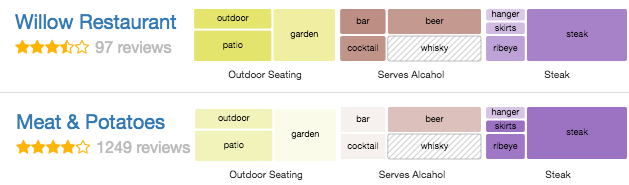
\includegraphics[width=1\columnwidth]{figures/explain.png}
%    \caption{}
%    \label{fig:explain}
%\end{figure}

\subsubsection{Keyword Suggestions}

\begin{figure}
    \centering
    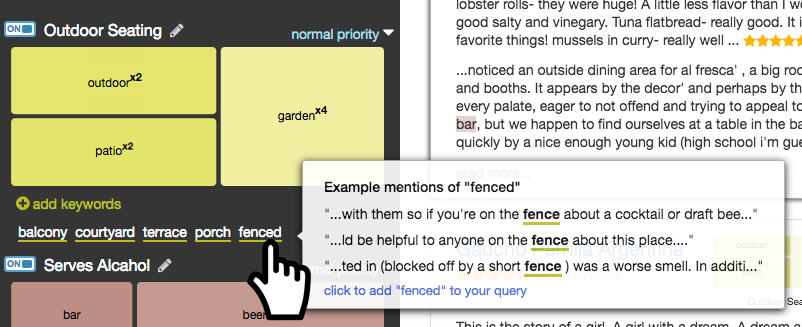
\includegraphics[width=0.6\columnwidth]{Chapters/SearchLens/figures/suggestions.png}
    \caption[SearchLens provides keywords suggestions based on currently Lenses.]{SearchLens provides keywords suggestions based on currently Lenses. Hovering shows a preview panel with mentions of the suggested keyword, allowing users to better understand the effect of adding the suggested keyword. In this case, SearchLens suggested balcony, terrace, fenced, and other keywords for the ``Outdoor Seating'' Lens. However, further inspection showed that fenced may not be a indicative keyword for the purpose of this Lens.}
    \label{fig:sl_suggestion}
\end{figure}


While creating a new Lens, listing all keywords from prior knowledge can be mentally taxing and have poor recall. To further reduce the required effort for building expressive Lenses, SearchLens generates Lens-specific keyword suggestions. As an example, when a user created an ``Outdoor Seating'' Lens with only three keywords (``outdoor'', ``patio'', and ``garden''), SearchLens automatically suggested relevant keywords including ``balcony'', ``courtyard'', and ``terrace'' (Figure~\ref{fig:sl_suggestion}). To do so, we trained a Word2Vec model \cite{mikolov2013efficient} with 300 dimensions using the entire Yelp dataset of 2,577,298 reviews. The trained word model can project words onto a semantically meaningful vector space, which in turn allows for measuring semantic similarity between words. Alternatively, it can also be used to find a set of words that are semantically similar to a given term by searching in the vector space of nearby words. To generate Lens-specific keyword suggestions, we first project all its keywords in a Lens onto the vector space and calculate the average vector to obtain a list of similar terms around the average vector. To further increase the chance of presenting useful and discriminatory search terms, we only used terms that appeared more than 50 times in the corpus, were mentioned in reviews of more than three restaurants, and were mentioned in less than 40\% of all restaurants.


\subsection{Interest-driven Explanation}

Persistent, decoupled user interest models would be beneficial to users the long run by providing separate reusable and recomposable interests across multiple search sessions. However, without immediate and perceivable benefits, users typically are not willing to spent extra effort expressing their separate interests for future tasks. For this, SearchLens uses each user's Lenses to provide visual explanation of each item in the search results. This is based on our approach of allowing users to express their multiple topics of interest separately, which enables SearchLens to distinguish between keywords of different topics and opens the possibility of visualizing each result according to users' interests in easy-to-interpret ways. Explanation is especially important for supporting searching with multiple interests, as it can be difficult for the users to understand which interests and keywords were associated with each result. Consider traditional search interfaces that only offer a short snippet for each result as explanation. These short summaries provide little support for personalized interpretation beyond a few highlighted query terms and their context. Even if users listed keywords of many different topics at once, the linear result list also provides little information about each result beyond their overall relevance ranking.

One obvious approach to explaining items in the search results is to surface mentions and statistical information, such as mention frequencies, at the topic level. For example, \cite{hoeber2006comparative} visualized the overall frequency of different search terms in different topics for each search result, and \cite{hearst1996visualizing} visualized the mention locations of different topics within each document. Visualizing at the topic level allowed these systems to provide mechanisms for specifying many topics and keywords, while at the same time visualized deeper information about each result in a way that matches the mental model of the searchers. However, visualizing at the topic level can be prohibitive for keyword-level operations, such as query reformulation and assigning importance levels to different keywords based on their frequencies.

\begin{figure}
    \centering
    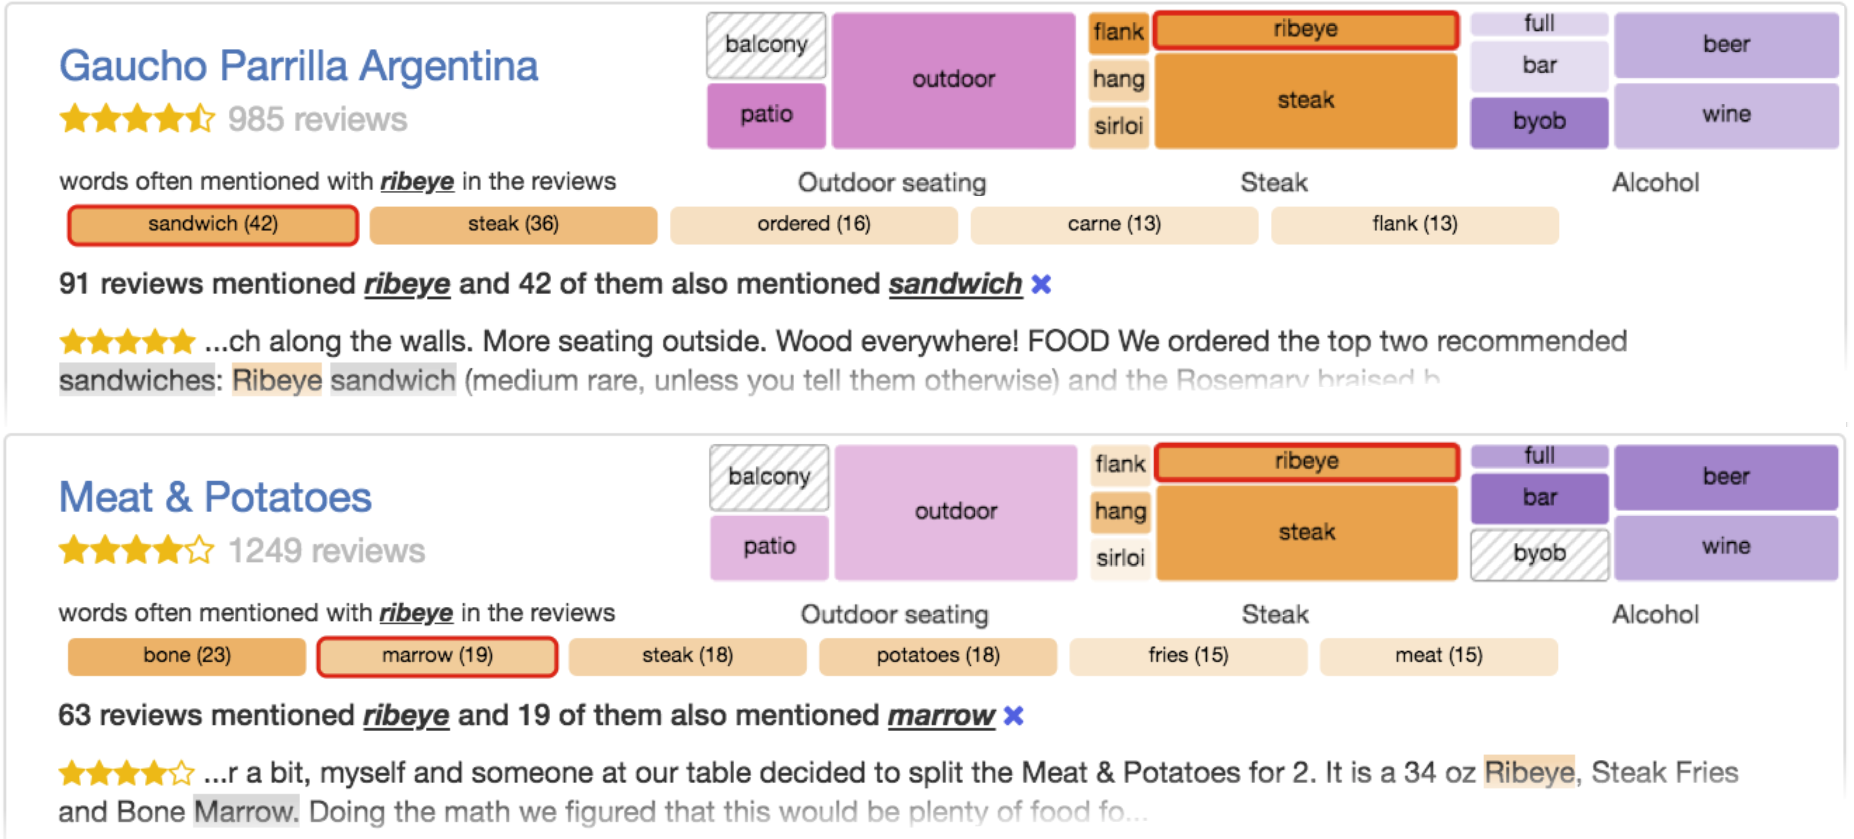
\includegraphics[width=0.8\columnwidth]{Chapters/SearchLens/figures/compare2.png}
    \caption[The visual explanation and exploration feature of SearchLens.]{The visual explanation and exploration feature allows comparison of results at different levels of granularity using a familiar interface used for specifying queries - at the levels of Lenses, keywords, co-occurring terms, and mentions, allowing users to query with multiple Lenses at the same time, while still being able to comprehend how each result matches their different Lenses.}
    \label{fig:sl_compare}
\end{figure}


% TODO messy -- should be fixed @nhahn thanks! @joseph
SearchLens supports rich explanation at the topic and keyword level through its user-specified Lenses. Explanation occurs by showing the each Lens visualization from the Query Panel (Figure~\ref{fig:sl_flow}) on each result and adjusting the term shading to correspond to the frequency of the term within that search result (Figure~\ref{fig:sl_compare}). By using identical colors and layouts of each Lenses, and showing result-specific keyword frequencies, users can quickly interpret how each result matches with their different interests at both the topic and at the keyword level using a familiar visualization. As an example, Figure~\ref{fig:sl_compare} shows how a user might examine two restaurants in a search result list using her Lenses for ``Steak'', ``Alcahol'', and ``Outdoor Seating''. At the topic level, both restaurants matched well with her Steak Lens rendered in dark shades that incorporated her stronger preference for ``ribeye'' steak, and also also her other interests such as ``flank'' steaks. She can also see that the first restaurant matched her Outdoor Seating Lens better than the second one. Looking at the same Alcohol Lens at the keyword level, she can easily see that the two restaurants matched differently with her ``Alcahol'' Lens where the first one has many mentions of ``byob'' in the reviews and the second one with many mentions of ``beer'' and ``bar'' instead.

%the she can easily infer that both restaurants have no reviews that mentioned her ``whisky'' keyword, and that the second restaurant also has very few mentions of ``cocktail'' as it is rendered in a light shade.

Finally, to provide a more compact, higher-level, topic-centric overview of all restaurants in the search results, SearchLens collapses the colored cells for each Lens into a single cell similar to \cite{hoeber2006comparative}. The size of each cell to shows the overall frequencies of keywords in different Lenses for each result (Figure~\ref{fig:sl_flow}). This allows users to get a quick overview of restaurants in the search results, and compare different options at the topic level using the Overview Panel at the bottom.


\subsection{Supporting Deeper Exploration of Items}
 

In addition to acting as a visual explanation for each result, the cells in the visualization also act as a navigation tool for deep exploration at the keyword level. Users can explore mentions of different keywords by clicking on its corresponding cell and the summary will update in real-time to show a list of its mentions. In addition, the Lens also shows the top co-occurring words that were frequently mentioned near the selected keyword as overview and deeper navigation, a strategy found useful in exploratory scenarios by prior work \cite{di2018study,di2016rank,peltonen2017topic}. As an example, Figure~\ref{fig:sl_compare} shows the how the Lenses allow users to explore and compare options at different levels of granularity. At the highest level, users can use the shading of different cells to see that the \emph{Outdoor Seating} Lens has more mentions in the first restaurant (Figure~\ref{fig:sl_compare}). Searchers can use the shading of individual cells to compare options at the keyword level. For example, the term ``BYOB'' was frequently mentioned in reviews for the first restaurant, but did not show up in reviews for the second restaurant. Finally, clicking on the individual cells allows users to explore mentions of its corresponding keywords and words that were frequently mentioned together. For example, when exploring mention of the work ``ribeye'' for both restaurants, SearchLens shows that there were many mentions of ``sandwich'' near the word ``ribeye'' for the first restaurant, and many mentions of ``bone marrow'' near ``ribeye'' for the second restaurant (Figure~\ref{fig:sl_compare}).



\subsection{Indexing and Ranking}

Traditionally, faceted search systems typically combine factors from multiple facets for ranking using disjunctions (factors within facets, such as brands selected by the user on a shopping website) and conjuctions (factors between facets, such as brands and price ranges). In an early iteration of SearchLens, we tested using the Boolean OR operator between keywords within the same Lens, treating keywords within the same Lens as synonyms while ranking. However, users reported this approach lead them to restaurants that poorly reflected their Lenses, as some restaurants may have many mentions of few keywords in a Lens, but very few mentions of other keywords. Fundamentally, unlike faceted search systems, different keywords in the Lenses typically describe a criteria as a whole. For example, an authentic ramen Lens might contained keywords describing creamy bone broth and freshly made noodles. In this case, the different keywords combined represented what the user considered good ramen restaurants, instead of as alternate options in a facet (such as a set of preferred brands). In a later iteration, we switched to Okapi BM25 for ranking that used inverse document frequencies to weight keywords instead of eliciting importance rating from the users. However, users reported unable to construct Lenses that reflect their priorities and unable to construct expressive Lenses that lead to useful results. This lead to the current iteration where we used a modified version of the standard Okapi BM25 ranking function to combine keywords across Lenses \cite{robertson2009probabilistic}, which by default considers both term frequency and document frequency to rank documents similar to TF-IDF ranking function, but also adjust for the length of each documents.

We modify the Okapi BM25 ranking function to account for the importance levels specified by users in the following ways. By default, Okapi BM25 uses the inverse document frequencies to weight each keywords, with the motivation that words appearing in many documents tend to be less important. Since in SearchLens users can specify keyword importance using the interactive visual explanation, we instead weight each keyword according to their user-specified importance level. By default, SearchLens assume each Lens is equally important, and normalizes the weights of keyword $q$ in a Lenses $\ell$ in proportion to the user-specified importance level of all keywords $\acute{q}$ in search Lens $\ell$:

%\vspace{-4mm}
$$weight(q) = \frac{importance(q)}{
    \sum_{\acute{q} \in \ell}{importance(\acute{q})}
}$$
%\vspace{-4mm}

SearchLens then uses the normalized keyword weights in place of the inverse document frequency term in the Okapi BM25 ranking function, and the score of each document $d$ in the corpus for a set of Lenses $L$ is therefore:

%\vspace{-4mm}
$$score(d, L) = \sum_{\substack{\ell \in L \\ q \in \ell}}\frac{weight(q) * tf(d, q) * (k+1)} { tf(d, q) + k * (1 - b + b *|d| / avgDL)}$$
%\vspace{-4mm}

where $\ell$ is the different user-specified Lenses, $q$ is the different keywords in each Lens $\ell$, $tf(d,q)$ is the term frequency of keyword $q$ in document $d$, $|d|$ is length of the document $d$, and the constant $avgDL$ is the average document length in the corpus. We used the default parameters $k=1.2, b=0.75$ for Okapi BM25. Finally, we sum up the score of each Lens weighted by a coordination factor, which is the proportion of keywords in a Lens that has a non-zero document frequency. This modified version of the Okapi BM25 function can be easily translated to SQL queries for standard relational databases, or as a custom ranking function for the popular open sourced document retrieval engine Apache Lucene. This allows the SearchLens interface to be easily implemented using readily available tools that were already optimized for scaling and computational efficiency. Admittedly, more sophisticated ranking approaches may further improve the quality of results, but this simple method allowed us to explore the costs and benefits of providing reusable, re-composable, explanation-centric Lenses to users.


\subsection{Implementation Notes}


The backend of SearchLens was implemented in Python, using NLTK \cite{bird2004nltk} and gensim \cite{rehurek_lrec} for indexing and word semantic model, respectively. In the indexing phase, text in each review is lowercased, tokenized, and stemmed using the Word Punkt Tokenizer \cite{jurish2013word} and Porter Stemmer \cite{van1980new}. Stop words are filtered out. An inverted index that records the document and the offsets of the mentions of each word stems is computed and stored in a PostgreSQL relational database. The Flask Python framework was used for our HTTP server. We implemented front-end of the SearchLens prototype as a web-based system using Javascript (ES6) and the ReactJS GUI framework, and the interactive visualizations are implemented using the D3.js library. User-specified Lenses were stored on client-side using browser cookies, so that they are persistent for the searchers between multiple visits.

\section{Evaluation}

We evaluated SearchLens in two studies. First, we conducted a usability study in a controlled lab environment. Using predefined tasks, we tested the usefulness and usability of the system, as well as whether the visual explanation and exploration features provide enough benefit to encourage participants to express their rich and multifarious interests. Second, we conducted a field deployment study where participants use SearchLens for their own tasks. This allowed us to explore the benefits and limitations of our reusable and re-composable Lenses in real-life scenarios.

%We evaluated SearchLens by conducting a lab study with 29 participants, and a field study with 5 participants. The studies aimed at assessing both the usefulness of the interface, and how searchers utilizes the different novel features and query paradigm. For the lab study, participants were given three predefined search tasks and personas, where we observe their strategies and behaviors on building and reusing the Lenses. For the field study, participants conducted their own search tasks outside the lab, so we can test SearchLens in real-life scenarios. During the studies, we logged the user interactions for further analysis. In the following subsections, we will describe the two studies in detail.



\begin{figure}
    \centering
    \frame{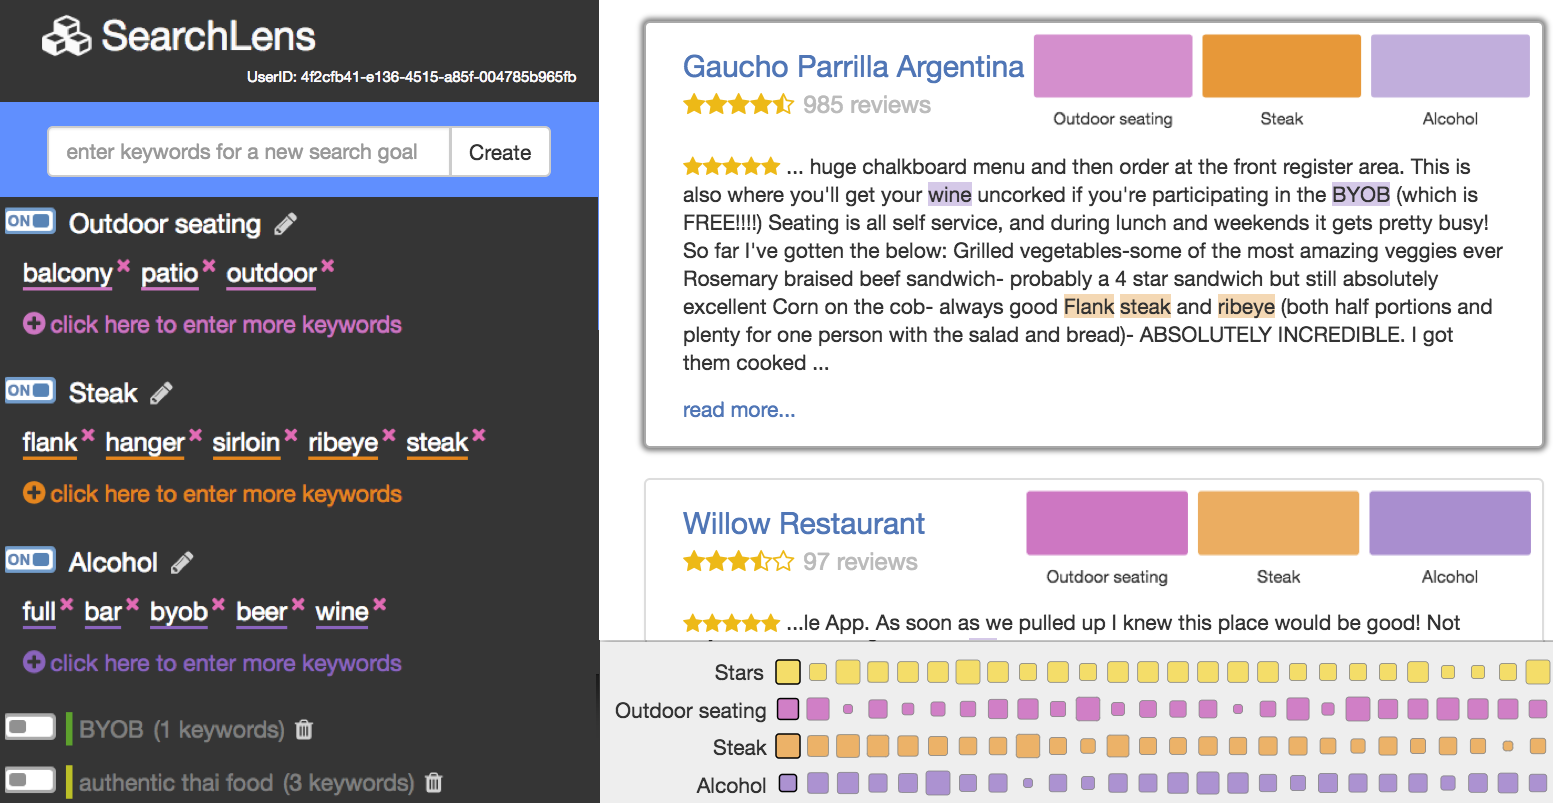
\includegraphics[width=0.8\columnwidth]{Chapters/SearchLens/figures/baseline3.png}}
    \caption[Baseline system interface for the SearchLens lab study.]{A Baseline system with topic-level visual explanation by collapsing the colored cells in each Lens and visualizing results only at the topic level.} %Unlike in the SearchLens condition, users can only explore each restaurants at the topic-level, but not the individual keyword level.}
    \label{fig:sl_baseline}
\end{figure}


\subsection{Usability Study}

The main goal of the usability study was to verify in a controlled lab environment the usability of the interface and whether the visual explanation and exploration features can provide benefits to encourage users to express their nuanced and multifarious interests. We considered these the preconditions for conducting a field deployment study to test the real-life benefits of reusable and re-composable Lenses. Therefore, we focused on the following:

\begin{itemize}
%    \setlength\itemsep{-2pt}

    \item whether the interface encouraged participants to externalize multiple interests and structure them using Lenses
    \item whether participants found the visual explanation and exploration feature to be useful 
    \item whether the added benefits of visual explanation and exploration encouraged participants to spend more effort to express, iterate, and refine their Lenses
\end{itemize}

To test the above, we compared SearchLens to a baseline interface as a between subject condition, where the detailed visual explanation and exploration features were removed by collapsing the colored cells in each Lens and visualizing results only at the topic level (Figure~\ref{fig:sl_baseline}), resulting an interface similar to the TileBars and the HotMap systems \cite{hearst1996visualizing, hoeber2006comparative}. Unlike in the SearchLens condition, users can only explore each restaurants at the topic-level, but not at the individual keyword level. Since searchers can not assign importance levels for each keyword in the baseline interface, we used the standard Okapi BM25 ranking function that weights keywords based on inverted document frequencies \cite{robertson2009probabilistic}. We chose this baseline as a more conservative test of the interactive explanation features than, for example, a comparison to Yelp or other search query-driven site (which are the implicit comparisons for the field study below).

The three scenarios for the usability study are listed below. The first scenario was designed to have both clear criteria (nice decor and good atmosphere and serves beer or wine), and an exploratory aspect (find a specific type of Japanese restaurant based on your own preferences). Scenarios 2 and 3 were designed to explore whether users would be able to reuse their Lenses for different contexts and find value in doing so. Scenario 2 had overlapping criteria to Scenario 1 (serves beer, cocktails, or wine), and Scenario 3 involved performing an identical search to Scenario 1 but in a different city.

\begin{itemize}
  
%  \setlength\itemsep{-4pt}
  
    \item \textbf{Scenario 1}: Stanley is in Pittsburgh, USA visiting some friends and he is in charge of finding a few good restaurants for the group. They are interested in Japanese restaurants. They're not familiar with Japanese food or the different types of Japanese restaurants, so it is up to you to find Japanese restaurants based on reading the reviews and your personal preferences. The restaurants should have a nice decor and good atmosphere. Some of his friends like to have a few drinks with their meal, so if the place has a bar that serves beer or wine it would also be great. Since its pretty nice out, it would also be nice if the restaurants has outdoor seating or a patio, too.
    
    \item \textbf{Scenario 2}: John is looking for good seafood restaurants in Pittsburgh, USA, particularly places that serves fresh oysters and has a bar that serves beer, cocktails or wine. Decor or atmosphere are not important, but big plus if they offer outdoor seating, for example, a patio. Some of his friends are allergic to seafood, so the place must also have non-seafood options, preferably steak.
    
    \item \textbf{Scenario 3}: (Same as Scenario 1 but for finding restaurants in Montreal, Canada instead of in Pittsburgh, USA.)
\end{itemize}

A total 29 participants were recruited from a local participant pool, where 14 participants were randomly assigned the SearchLens interface with three predefined search tasks (N=14, Age=18-61, M=28.1, SD=12.7, 7 male, 6 female, and 1 other/not listed), and 15 participants assigned the baseline interface with the same search tasks (N=15, Age=18-54, M=28.1, SD=10.7, 7 male, 7 female, and 1 other/not listed). Each participant was given 60 minutes to complete the study and was compensated 10 USD. Before conducting the three tasks, participants watched a five minute introduction video that described the features in their given interfaces, which is followed a step-by-step training where participants created two pre-defined Lenses, report the name of the third restaurant in their search results, and report which keyword is missing from its reviews. Participants finished the training steps using an average of 5.9 minutes (N=29, SD=3.8). For the main task, participants were told to spend 10 to 15 minutes on each of the three tasks listed above in order. Finally, participants answered a short post-survey where we collected their subjective opinions about the systems using 7-point Likert scales and free-form responses.


%\begin{figure}[]
%    \centering
%    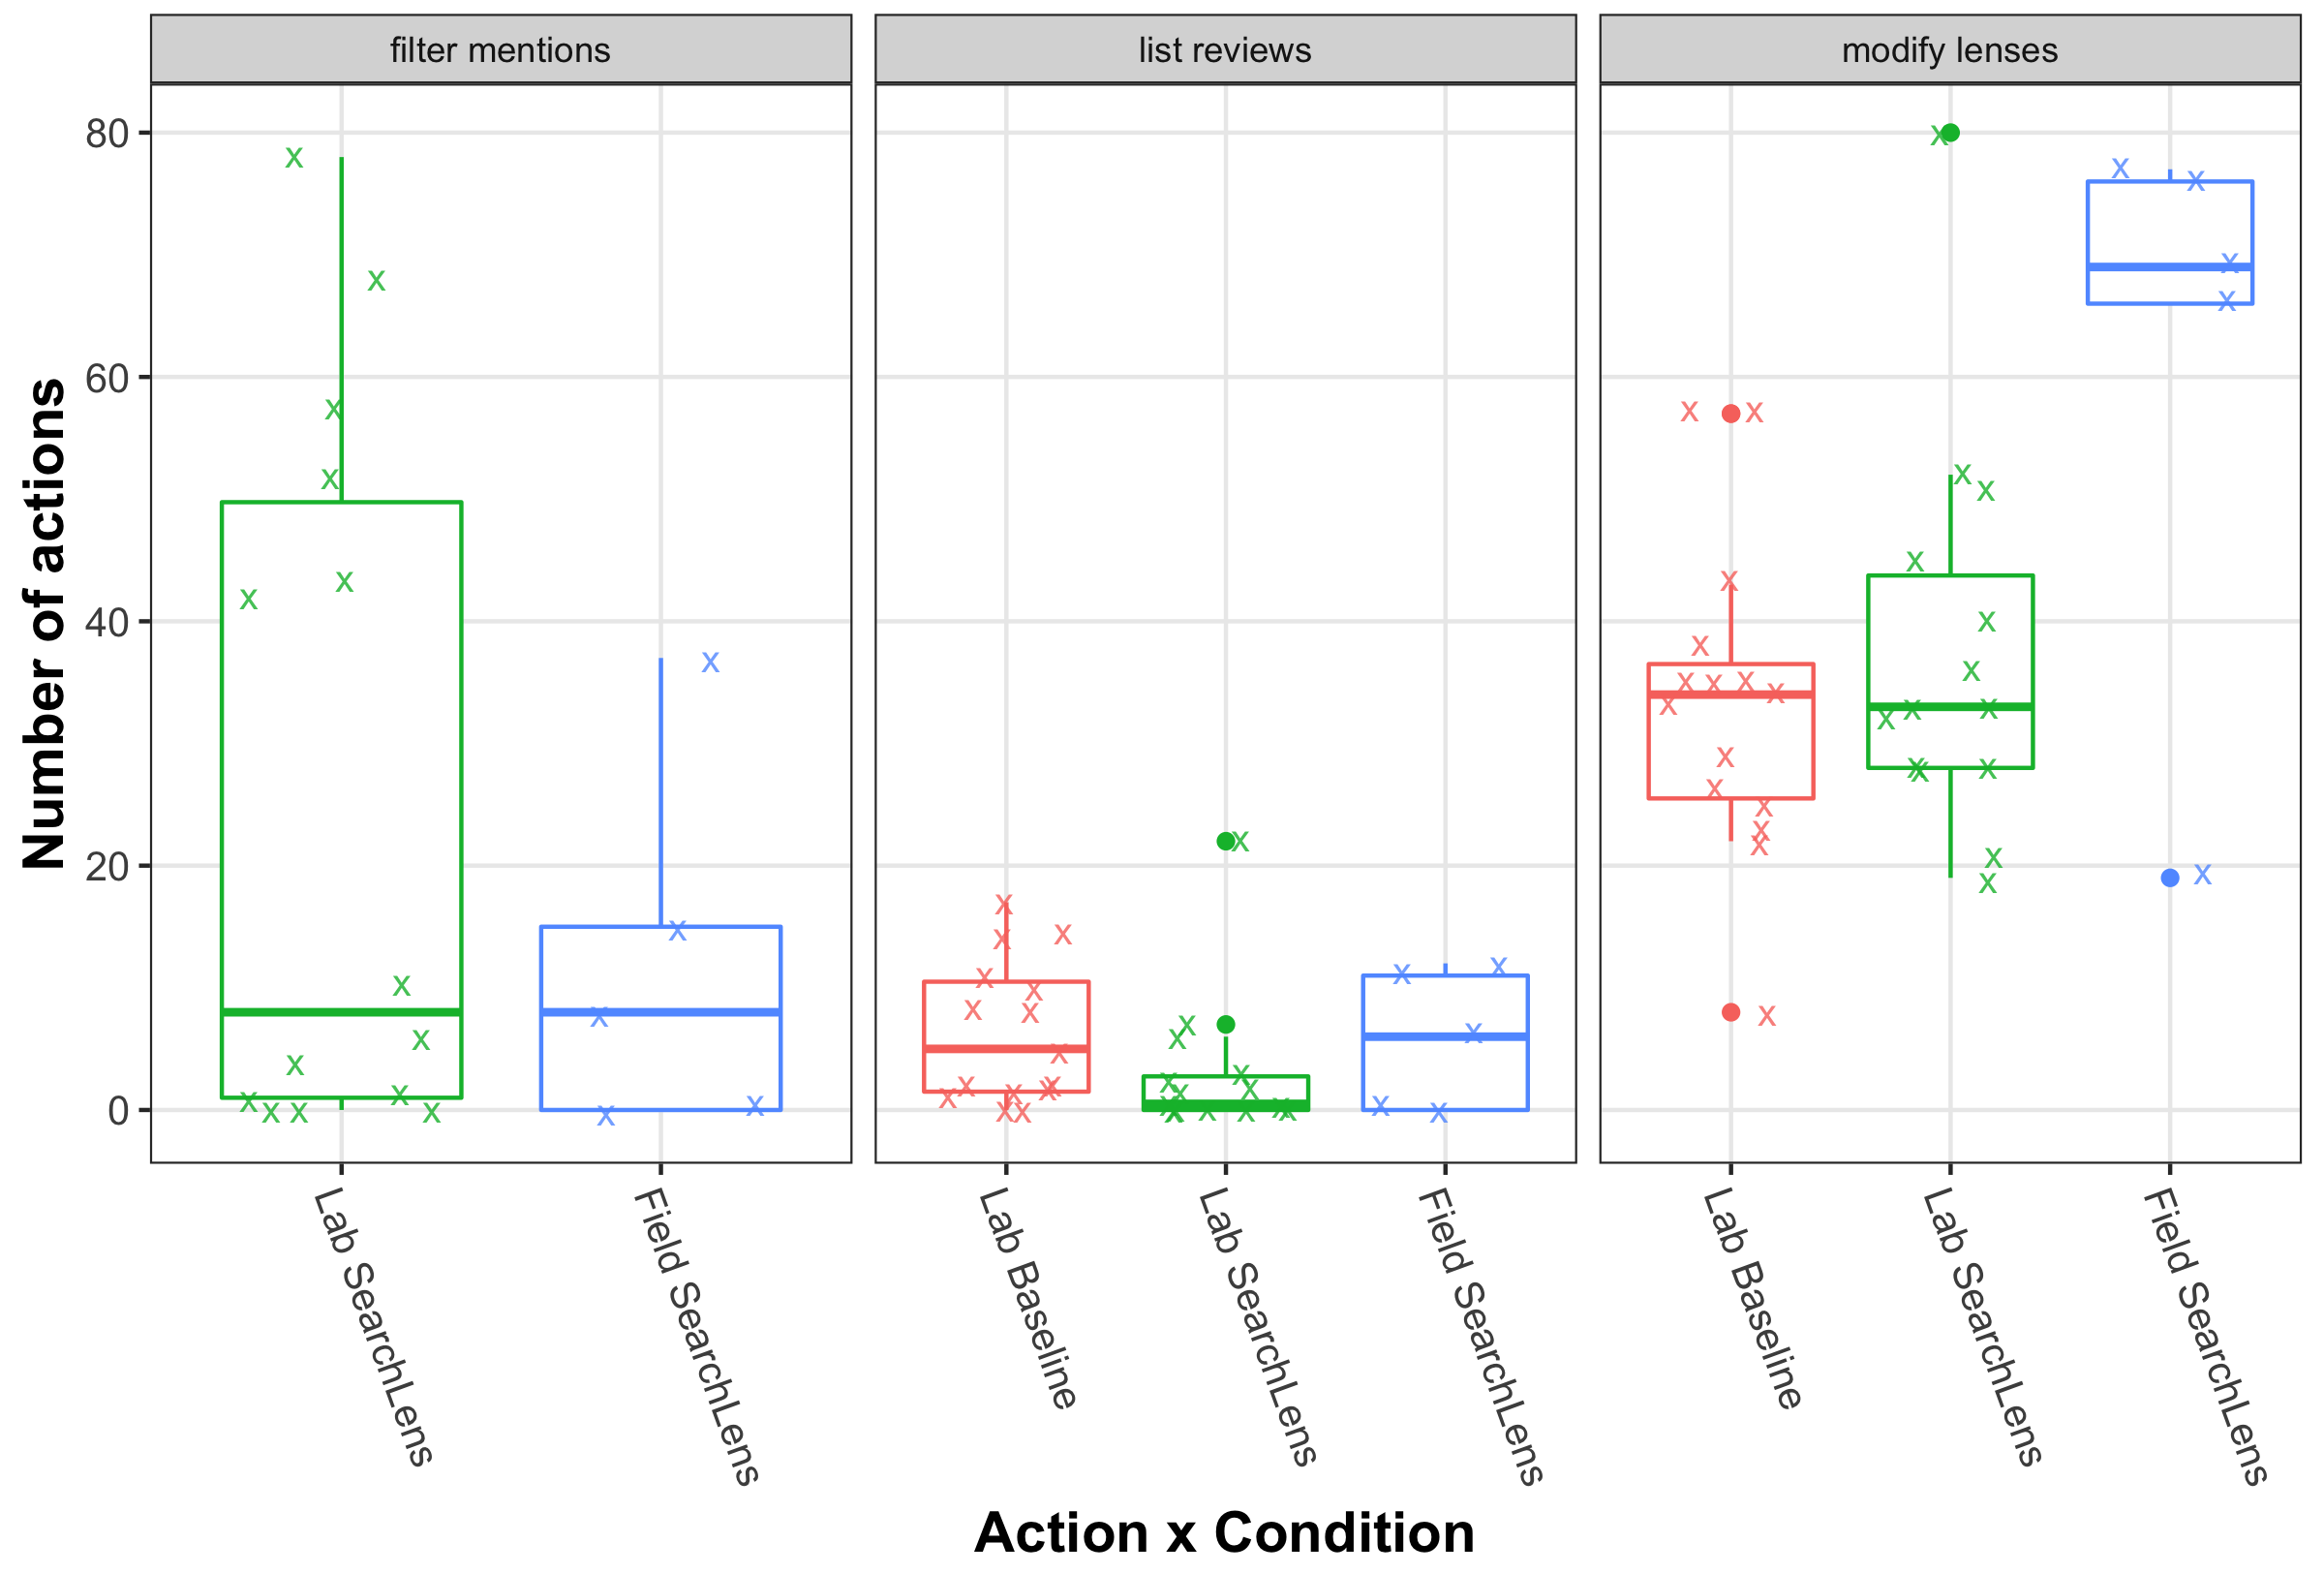
\includegraphics[width=1\columnwidth]{figures/Behavior.png}
%    \caption{Number of different action participants performed under %different conditions. Participants in Baseline relied on reading full %reviews to understand results, whereas participants SearchLens %frequently used the interactive treemaps to see keyword mentions. %Participants conducting their own tasks in the Field study tend to %refine their Lenses often.}
%    \label{fig:behavior}
%\end{figure}



%\subsubsection{Expressing Interests with Lenses}


%As a usability check, we first examine if participants expressed different interests using multiple Lenses instead of simply creating a single lens of multiple interests (analogous to a single search query bar). Figure~\ref{fig:sl_numberOfLenses} and~\ref{fig:sl_counts} show the number of Lenses each participants have saved at the end of the study, and in both conditions participants created multiple Lenses. On average, participants created 7.64 Lenses in the SearchLens condition (N=14, SD=3.65), and 6.54 Lenses in the baseline condition (N=15, SD=2.37). No significant difference was found between conditions based on unpaired T-Test (t(27)=0.94, p=0.36). This was expected since the predefined scenarios had many clearly defined criteria, and participants generally created one lens for each criteria (with multiple terms nested within lenses).

\begin{figure}
    \centering
    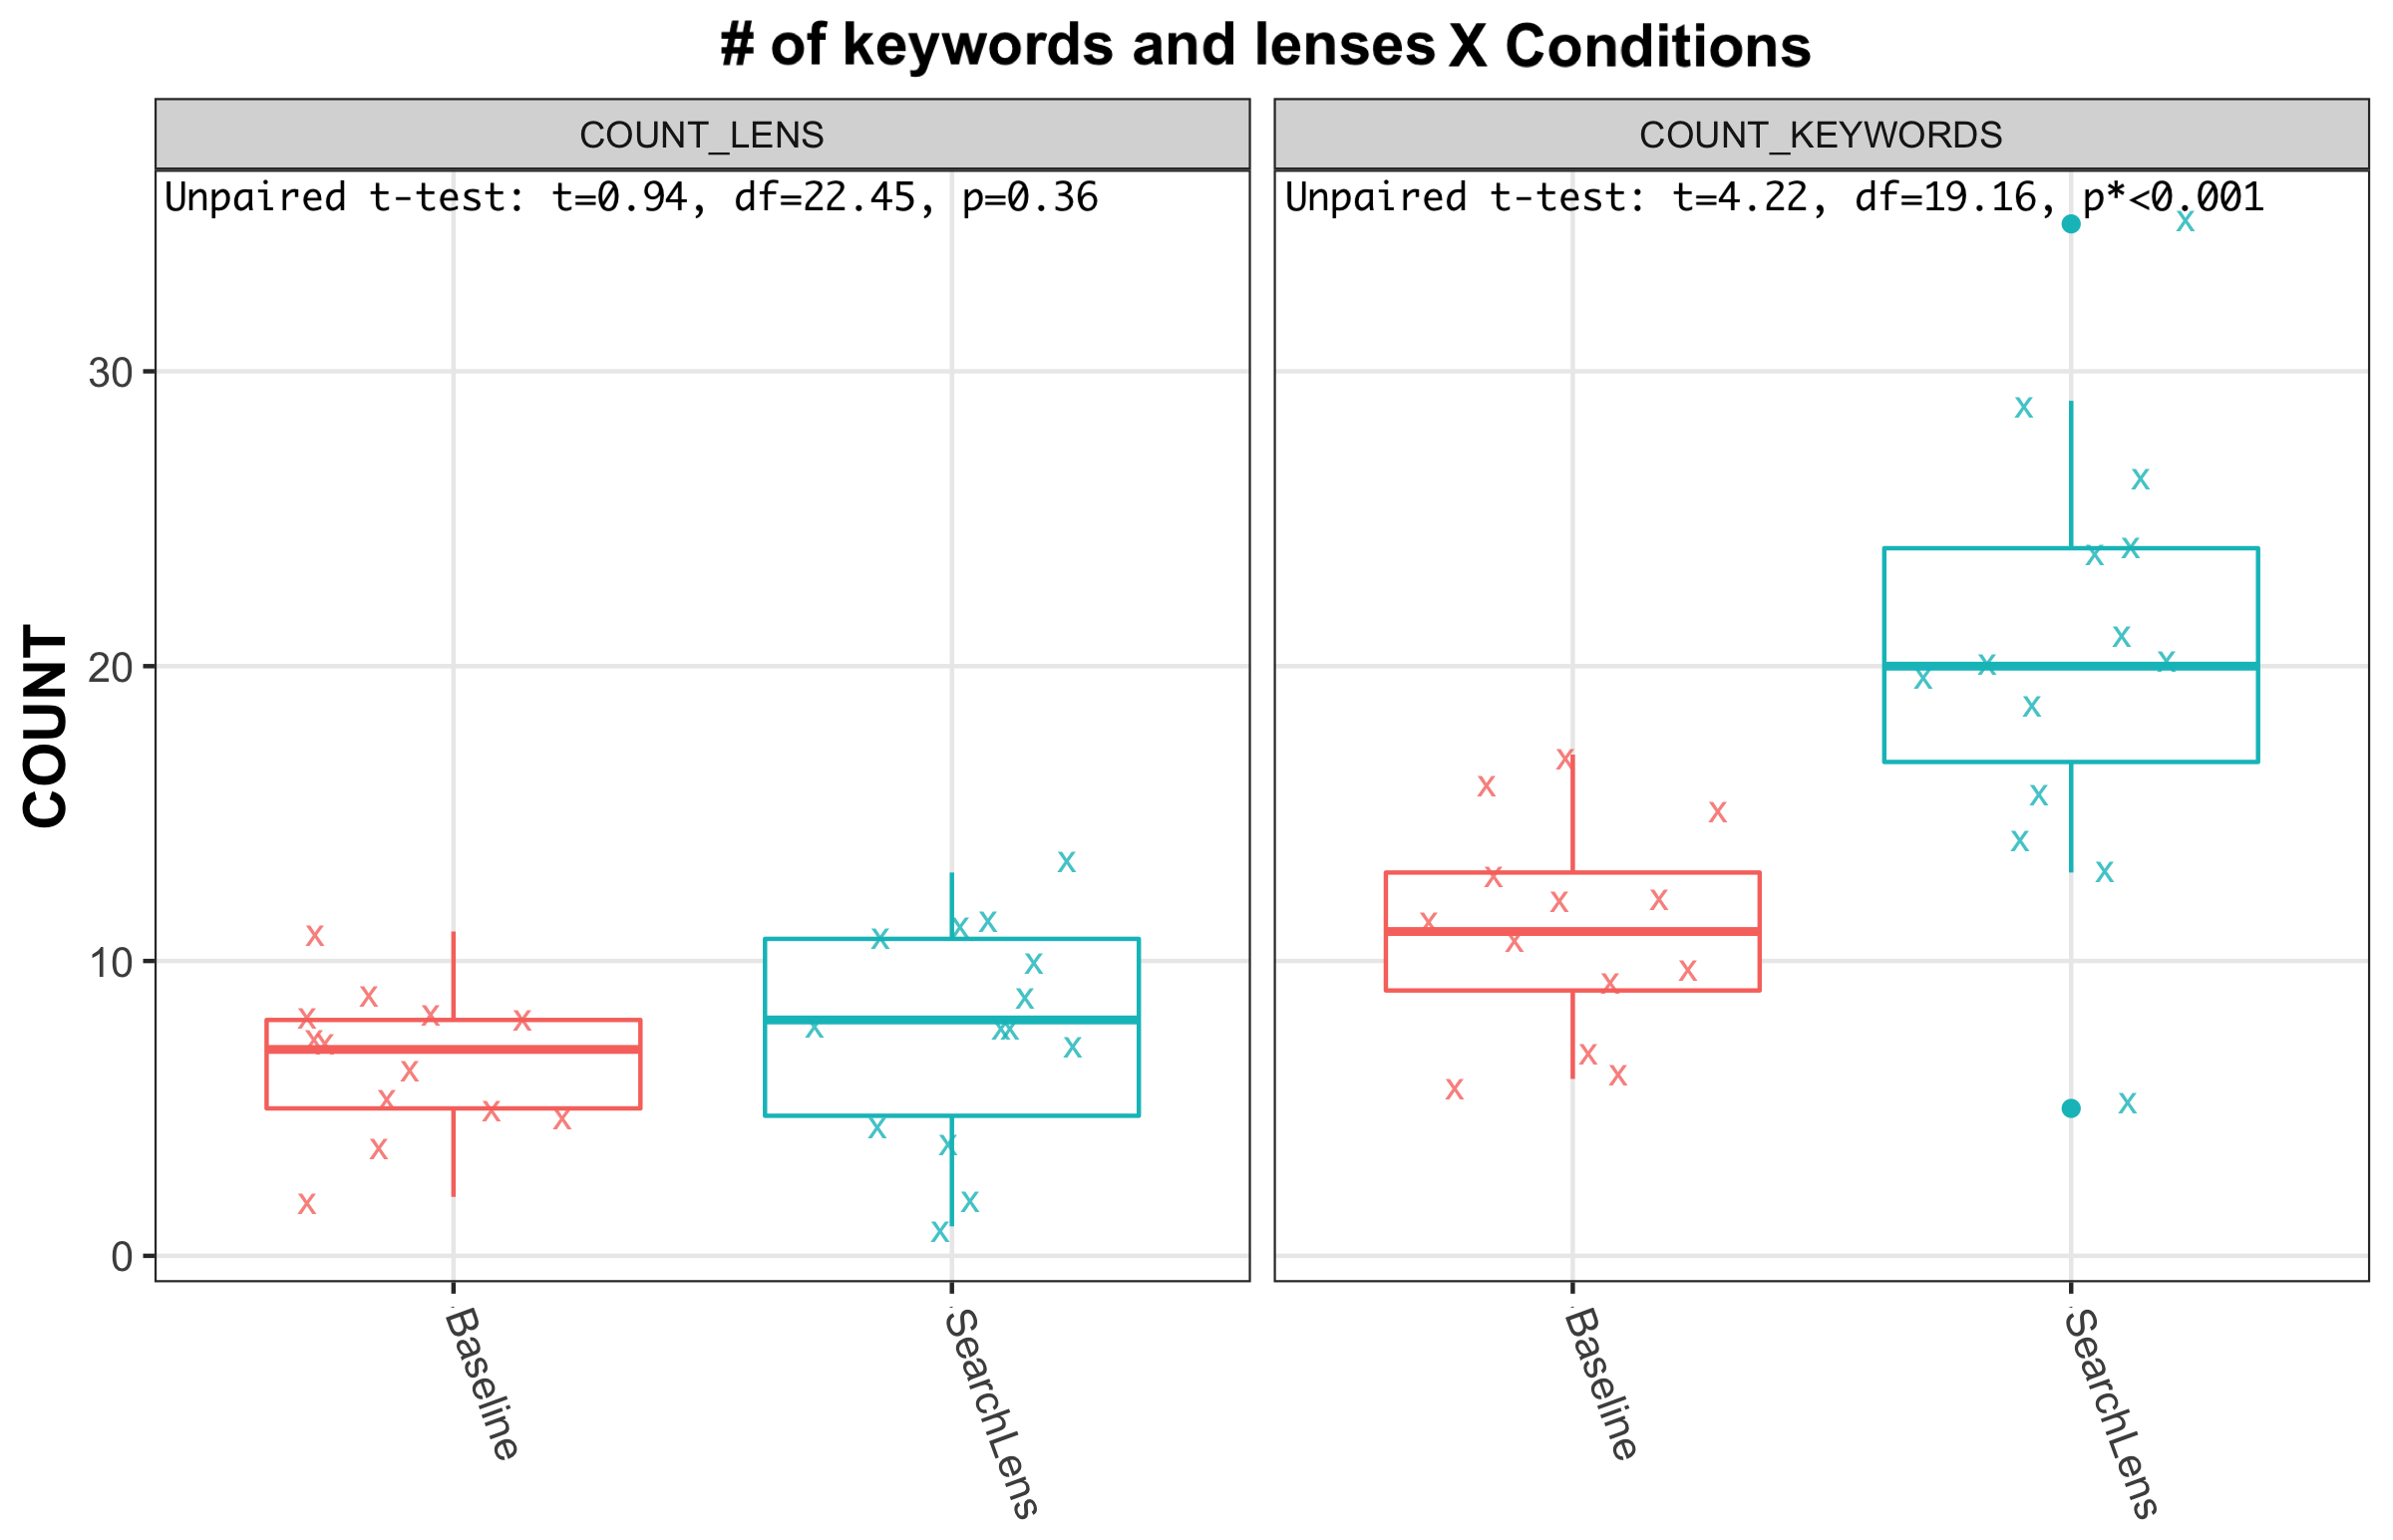
\includegraphics[height=0.45\columnwidth]{Chapters/SearchLens/figures/LensKeywordsCount3.png}
    \caption[Number of Lenses and keywords saved the participants.]{Number of Lenses and keywords saved by each participants at the end of the study. Participants in both conditions created comparable number of search Lenses, but participants in the SearchLens condition collected significantly more keywords in their Lenses.}
    \label{fig:sl_numberOfLenses}
\end{figure}

\begin{table}
  \centering
  \small

\setlength\tabcolsep{4pt} % default value: 6pt

  \begin{tabular}{ r | r l | r l |  r l }
  
	&
	\multicolumn{2}{c}{Lab} &
	\multicolumn{2}{c}{Lab} &
	\multicolumn{2}{c}{Field} \\
	
	Action &
	\multicolumn{2}{c}{Baseline} &
	\multicolumn{2}{c}{SearchLens} &
	\multicolumn{2}{c}{SearchLens} \\
    
	\hline
	
    
	 %add a new lens &
     %12.53 & $\sigma$=5.25 &
     %9.64 & $\sigma$=4.48 &
     %13.80 & $\sigma$=7.09 \\
     
	 add terms by typing &
     3.67 & $\sigma$=2.82 &
     5.50 & $\sigma$=4.86 &
     7.00 & $\sigma$=5.39 \\
     
	 add from suggestions &
	\multicolumn{2}{c|}{n/a} &
     1.57 & $\sigma$=1.99 &
     3.20 & $\sigma$=1.79 \\
     
	 add from reviews &
	\multicolumn{2}{c|}{n/a} &
     0.29 & $\sigma$=0.73 &
     0.40 & $\sigma$=0.55 \\
     
     \hdashline[1pt/1pt]
     
	 total add actions &
     3.67 & $\sigma$=2.82 &
     7.36 & $\sigma$=6.10 &
     10.60 & $\sigma$=3.71 \\
     
     \hline
     
     
	 remove a keyword &
     4.67 & $\sigma$=4.27 &
     3.50 & $\sigma$=2.79 &
     4.20 & $\sigma$=2.68 \\
     
	 adjust weights &
	\multicolumn{2}{c|}{n/a} &
     8.93 & $\sigma$=7.54 &
     12.80 & $\sigma$=7.89 \\
     
	 %reuse a lens &
     %2.00 & $\sigma$=1.85 &
     %1.64 & $\sigma$=1.28 &
     %4.20 & $\sigma$=3.96 \\
	\hline
	
	&
	\multicolumn{2}{r}{N=15} &
	\multicolumn{2}{r}{N=14} &
	\multicolumn{2}{r}{N=5} \\
	
  \end{tabular}
  \caption[Number of Lens editing actions performed under different conditions.]{Mean statistics for number of Lens editing actions performed by participants. Participants used SearchLens in the lab study more frequently add keywords to refine Lenses compared to baseline (t(27)=2.12, p<0.05). Participants in the field study conducted their own tasks. }
  \label{tab:actions}
\end{table}



\subsubsection{Results for the Usability Study}

One of our key hypotheses was that the immediate visual explanation provided by Lenses would encourage participants to express their interests and continually collect and refine those interests throughout the search process. This hypothesis appears to have been validated by the data. On average, participants in the SearchLens condition saved 20.43 keywords across their Lenses (N=14, SD=7.33), significantly more than participants in the baseline condition who saved 11.15 keywords (N=15, SD=3.58; t(27)=4.12, p<0.001). Importantly, this difference is likely not attributable to different perceptions of the task across conditions, as in both the SearchLens and baseline conditions participants generally created one Lens for each task criteria and combined multiple Lenses for each task (e.g., decor, drinks) and there was no difference between the total number of Lenses created between conditions (SearchLens: 7.6, baseline: 6.5; t(27)=0.92, p=0.36). In other words, the term-based interactive visual affordances supported by SearchLens seemed to encourage people to collect more terms indicative of their interests.

This pattern appeared to hold true throughout the search process for the iterative refinement of Lenses as well (Table~\ref{tab:actions}). On average, participants using SearchLens added keywords to existing Lenses 7.4 times (N=14, SD=6.1) while those in the baseline condition did so 3.7 times (N=15, SD=2.8), which was found to be a significant difference (t(27)=2.12, p<0.05). This suggests that the added benefits from the visual explanation and exploration feature encouraged participants to iteratively refine their Lenses and allowed them to discover useful keywords more often.

We also examined whether participants found the added visual exploration features to be useful, and how the added benefits affected their behavior. By examining the behavior logs, we found participants using SearchLens frequently use the visual exploration feature. On average, each participant clicked on 25.86 (SD=29.19) keywords to filter reviews that mention a specific keyword instead of sifting through reviews to find ones that mentioned it (Figure~\ref{fig:sl_reviews}). In both conditions, participants can also click on the name of a restaurant to see a list of reviews ranked by all active Lenses. While there is suggestive evidence that the filtering of reviews led to less use of the generic review lists, the result was not significant based on the number of participants in the study (M=6.33, 3.07; SD=5.78, 5.92; t(27)=1.50; p=0.15).

% we found participants in the baseline condition list reviews of different restaurant more often than participants using SearchLens on average , but the difference was not significant


These results suggest SearchLens allowed participants to maintain a broader search goal with multiple interests, while at the same time explore and compare different options at a finer-grain level interactively instead of sifting through the reviews of each restaurant.


%These results suggest that the added benefits of visual explanation encouraged participants to express their rich and nuance interests and also encouraged them to iteratively refine their Lenses throughout the search process.






% \subsubsection{Visual Explanation and Exploration}


%Figure~\ref{fig:sl_counts} shows the number of Lenses and keywords each participants under different conditions collected during the study. In general, participants in either condition generated similar number of Lenses. This is expected since the predefined scenarios had many clearly defined criteria. However, results suggest 

%Figure~\ref{fig:behavior} shows the number of actions participants performed under different conditions. In general, participants in the Baseline condition examined the full review lists of different restaurant more frequently then participants in the SearchLens conditions. On the other hand, participants in the SearchLens condition frequently used of the interactive treemaps to filter out mentions of different keywords, which was not available to the participants in the Baseline condition. This suggests that participants in the Baseline condition relied on listing and reading full reviews in order to understand the search results, whereas participants in the SearchLens condition frequently used the interactive treemaps to see mentions of their different keywords in the reviews directly on the search results page. Participants under the two conditions performed similar number of lens modifying actions. Figure~\ref{fig:lens_behavior} shows the average number of detailed lens modifying actions. More than 70\% of the participants in either condition reused their Lenses across condition (with 11 out of 15 participants for the Baseline condition, and 10 out of 14 participants out of the SearchLens condition). Participants under the SearchLens condition used keywords from prior knowledge by creating Lenses and adding keywords to them, but also found keywords in the reviews and used the suggested keywords. In the Field Study, we examined in more detail on how searchers utilizes different SearchLens features to refine their Lenses.


%\begin{figure}[]
%    \centering
%    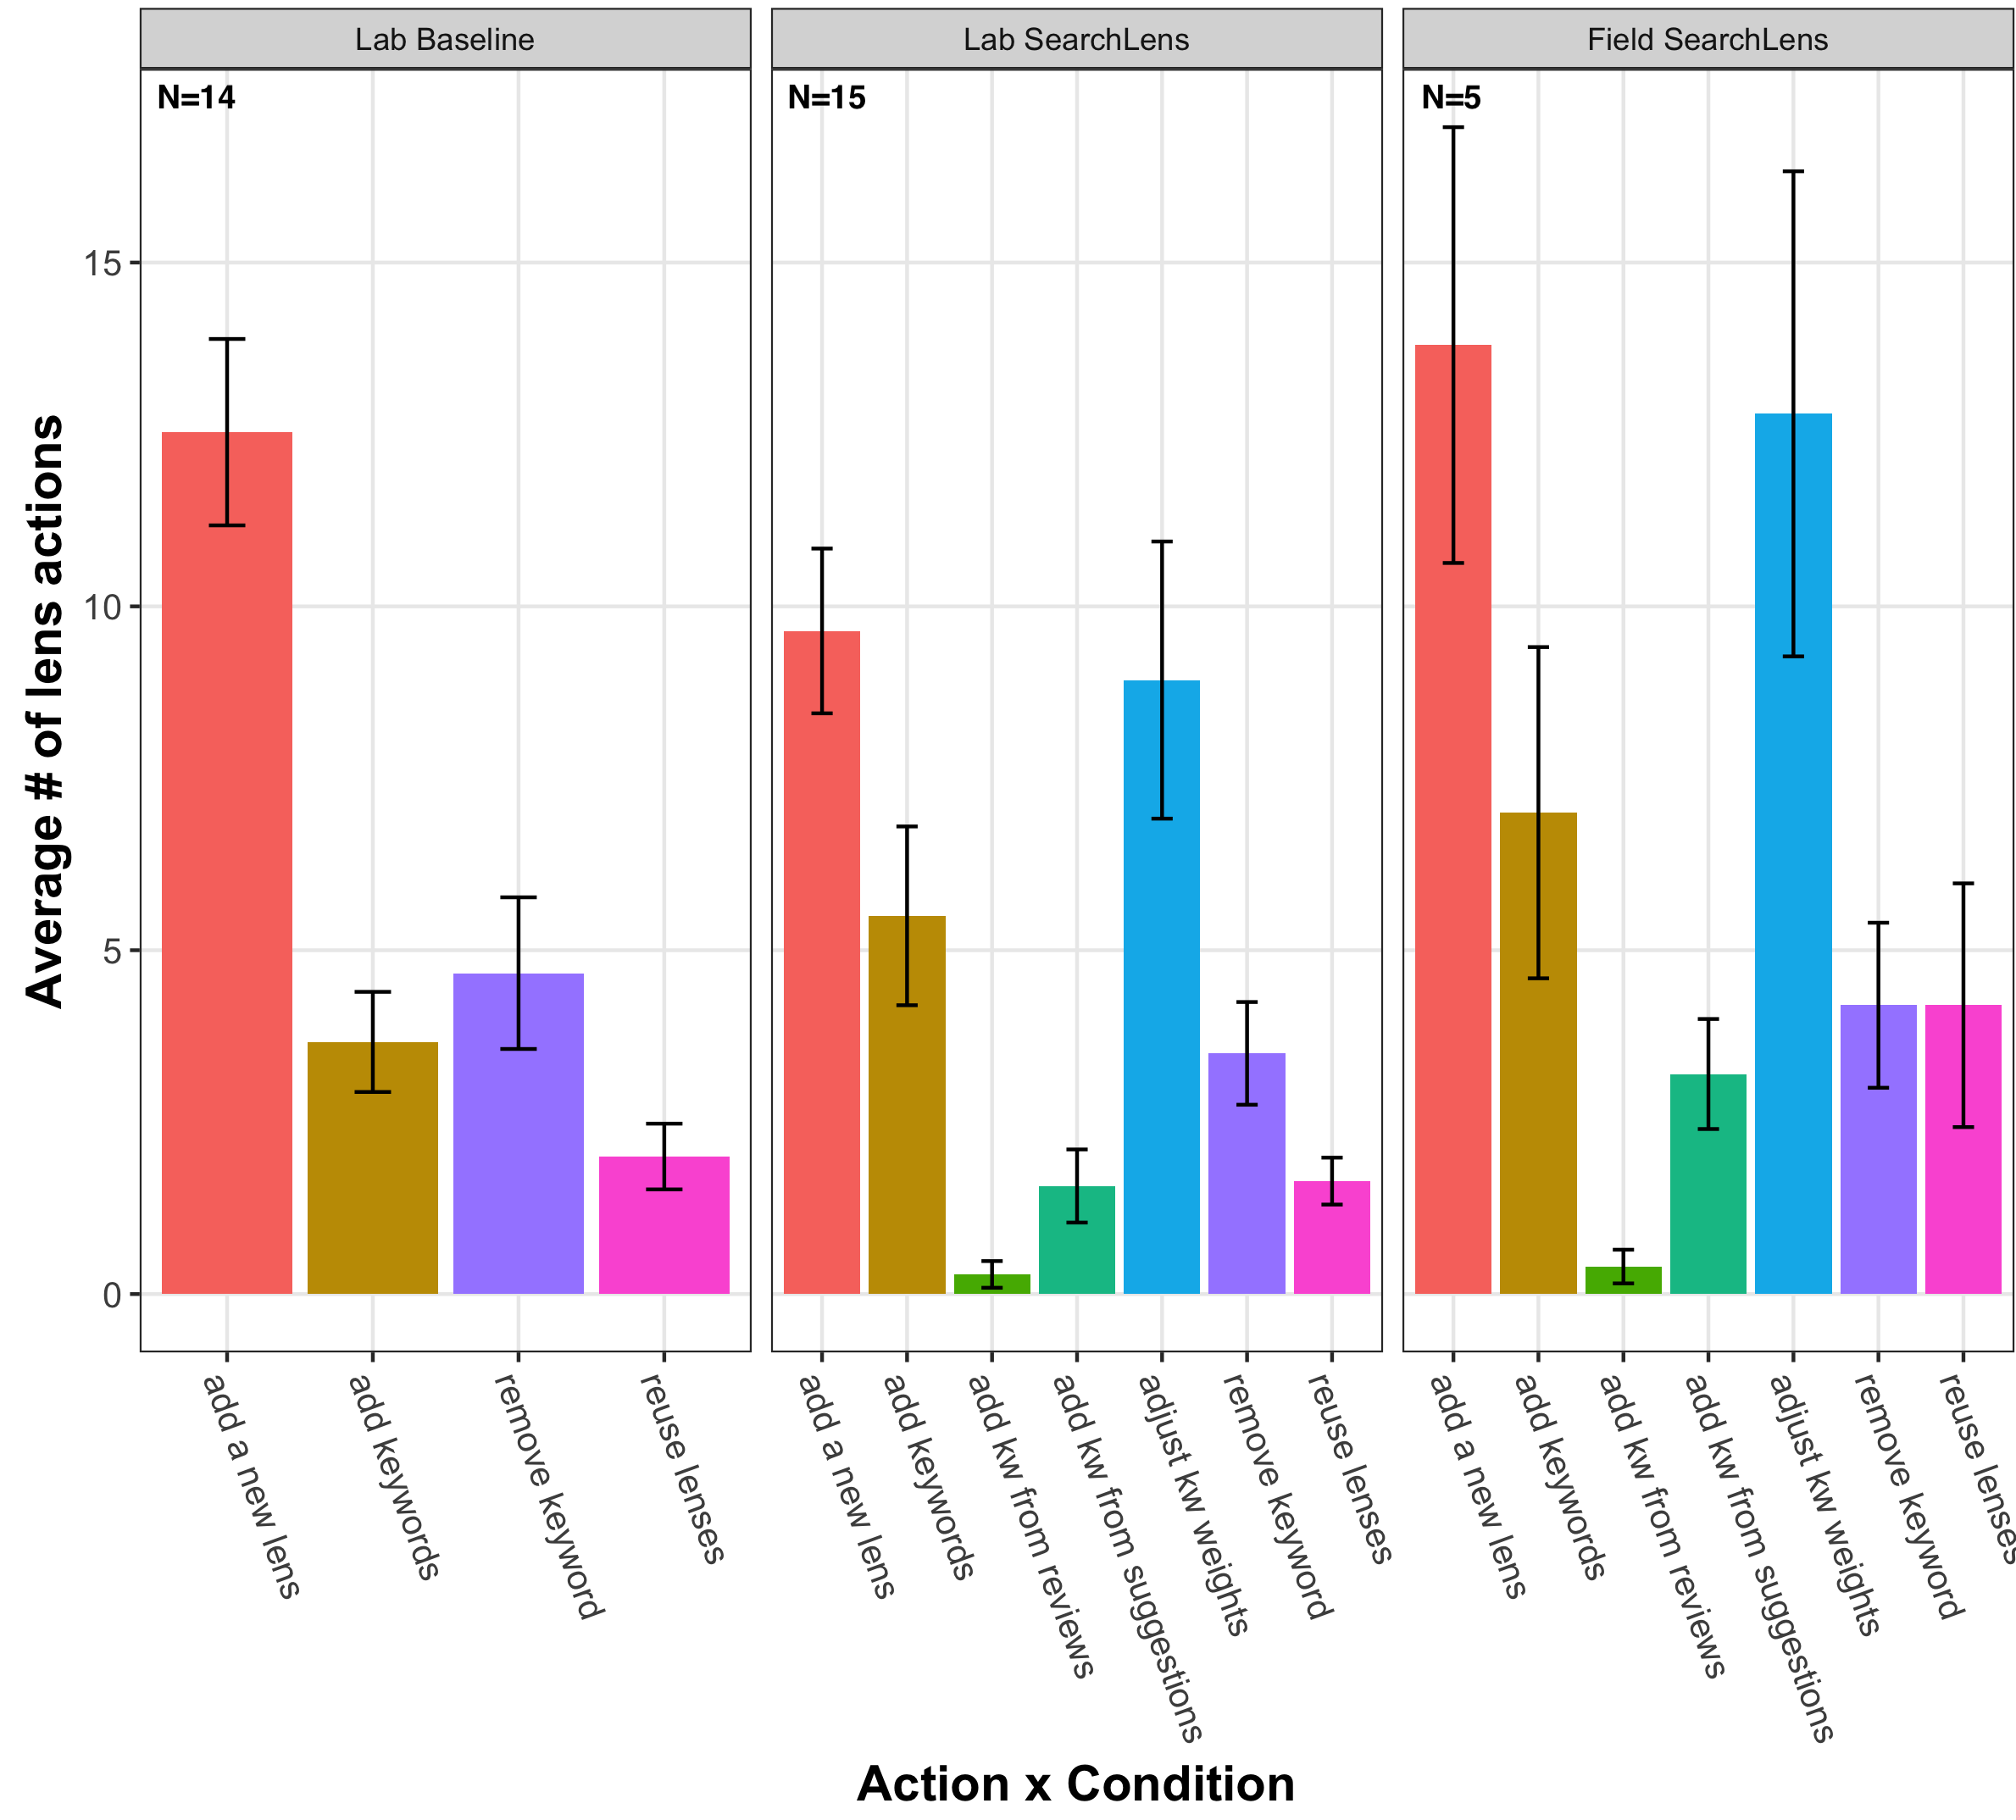
\includegraphics[width=1\columnwidth]{figures/LensBehavior2.png}
%    \caption{Average number of lens editing actions performed by participants under %different conditions. Notice keyword specific features are not available in the %Baseline condition.} %\adam{Minor: this chart is very hard to read, due to the %similar colors and overlapping text, and redundant key.  If there is time, might be %worth cleaning it up a bit.}}
%    \label{fig:lens_behavior}
%\end{figure}



%We designed the first and the third tasks to have overlapping criteria to see whether participants would reuse their Lenses created for the first task that may have been disabled while  performing the second task. Most participants in both condition re-enabled some of their Lenses that were created previously (baseline: 73.3\%, SearchLens: 71.4\%). Upon closer examination, we found that some participants deleted Lenses that were not relevant to the second task and had to recreate them for the third task, citing that they ``\emph{did not realize these are going to be useful for the third task}''. In the field study section, we further explored the benefits of reusable Lenses in real-world settings where participants conducted their own tasks using SearchLens.


% NOTE: What about combining and reusing lenses? We say that is something we wanted to look at in the usability study but I don't see anythign about it yet. Did people combine lenses?  Did they reuse their lenses when they had to do the search in a new city?


\begin{figure}
    \centering
    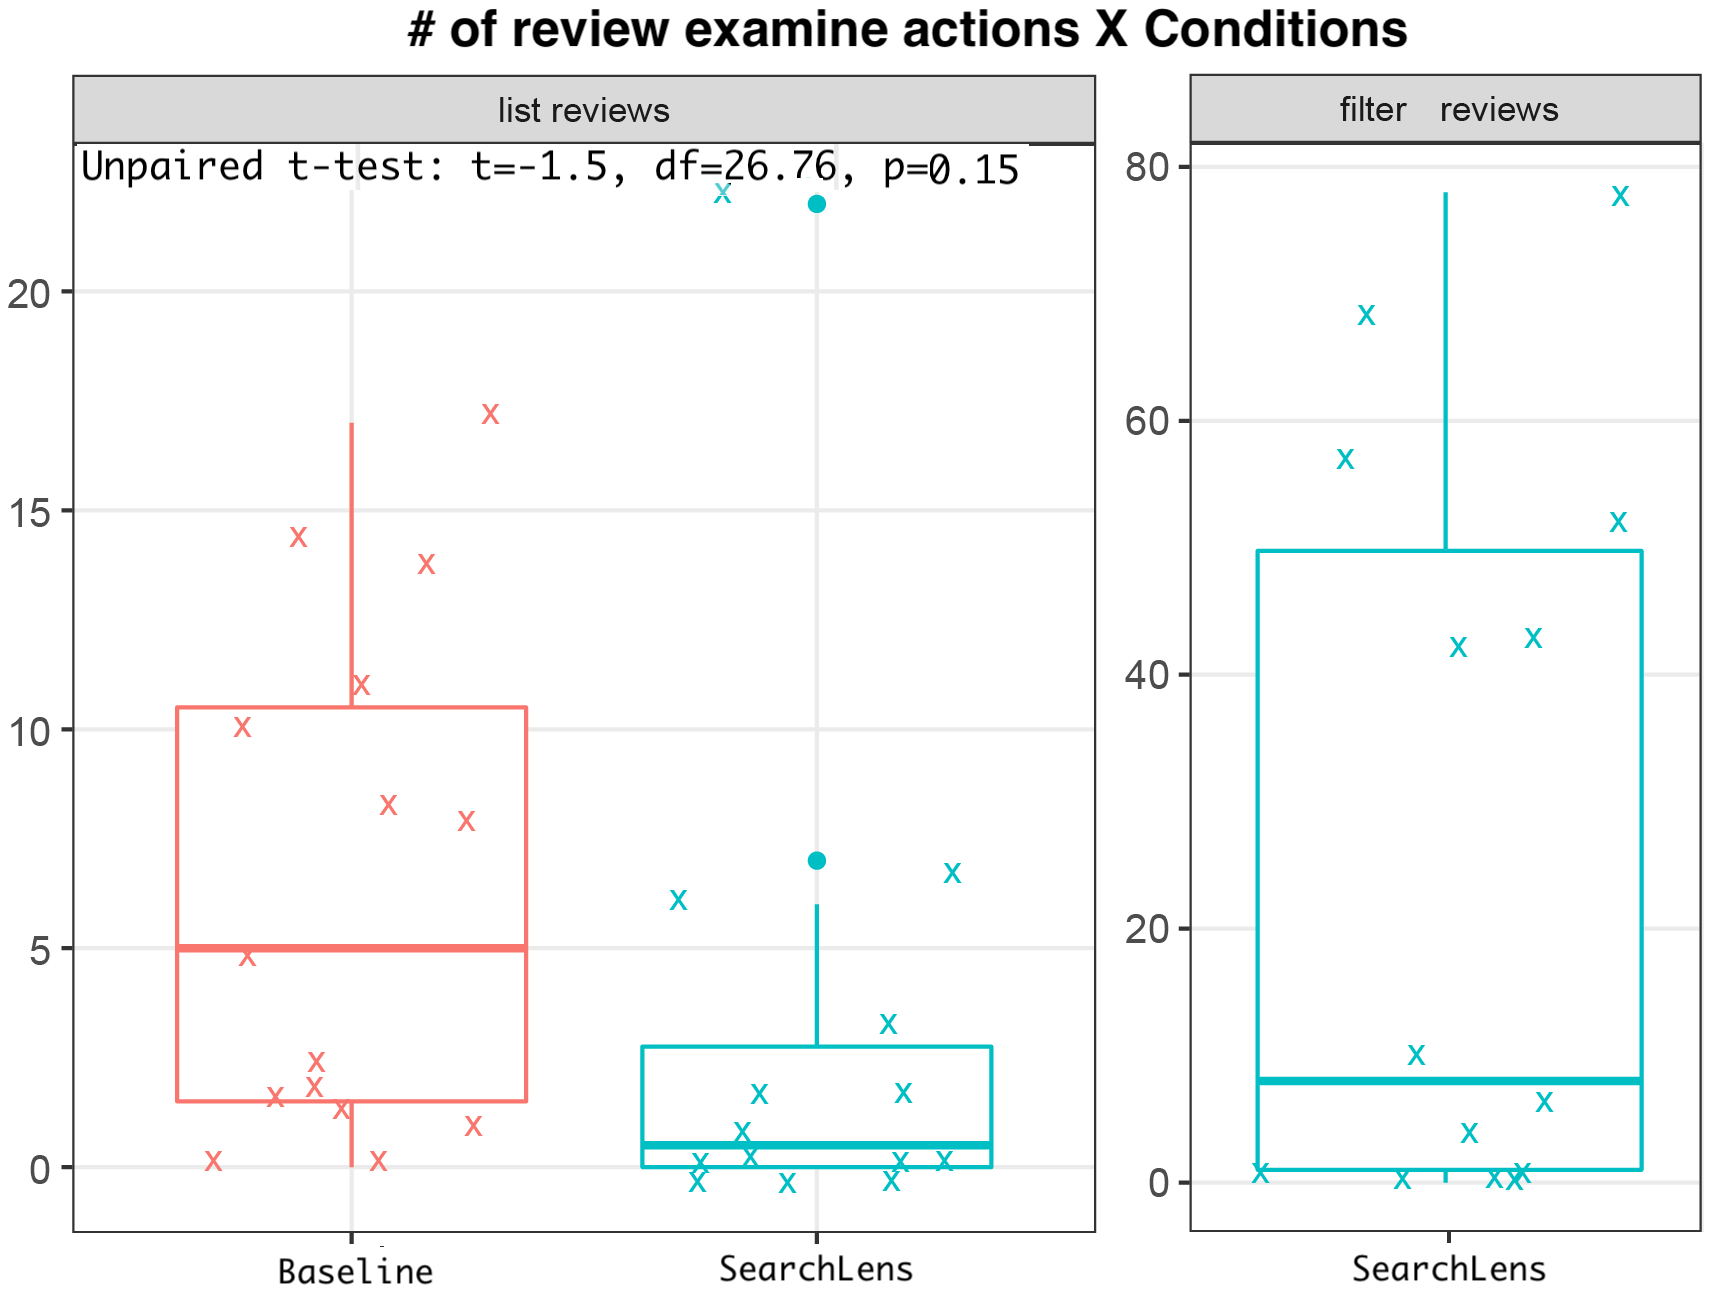
\includegraphics[height=0.45\columnwidth]{Chapters/SearchLens/figures/reviews.png}
    \caption[Participants frequently interactive with their Lenses instead of sift through reviews]{Participants in the SearchLens condition were less likely to read through unfiltered lists of reviews than the baseline condition, which was accompanied by increased use of the SearchLens-specific ability to filter reviews relevant to different keywords.}
    \label{fig:sl_reviews}
\end{figure}



\subsection{Field Study}

Our field deployment study aimed to test our idea of reusable and re-composable Lenses in real-world settings. Five participants were recruited from the first study based on their high self-reported interest in researching restaurants online and in participating in a follow up study (N=5, Age=18, 20, 22, 23, and 25, 4 male, and 1 others/not listed). The participants were given access to the SearchLens system via the internet, and were asked to use the system for at least 60 minutes in total over a three day period. Although they were free to choose from any of the 11 cities in the dataset for this study, all five participants conducted tasks for their current city.
Afterwards, they return to the lab and were given 45 minutes to finish a survey with primarily free-form questions, and were interviewed for another 15 minutes. Each participant was compensated with 40 USD for finishing the study.

\begin{figure}
    \centering
    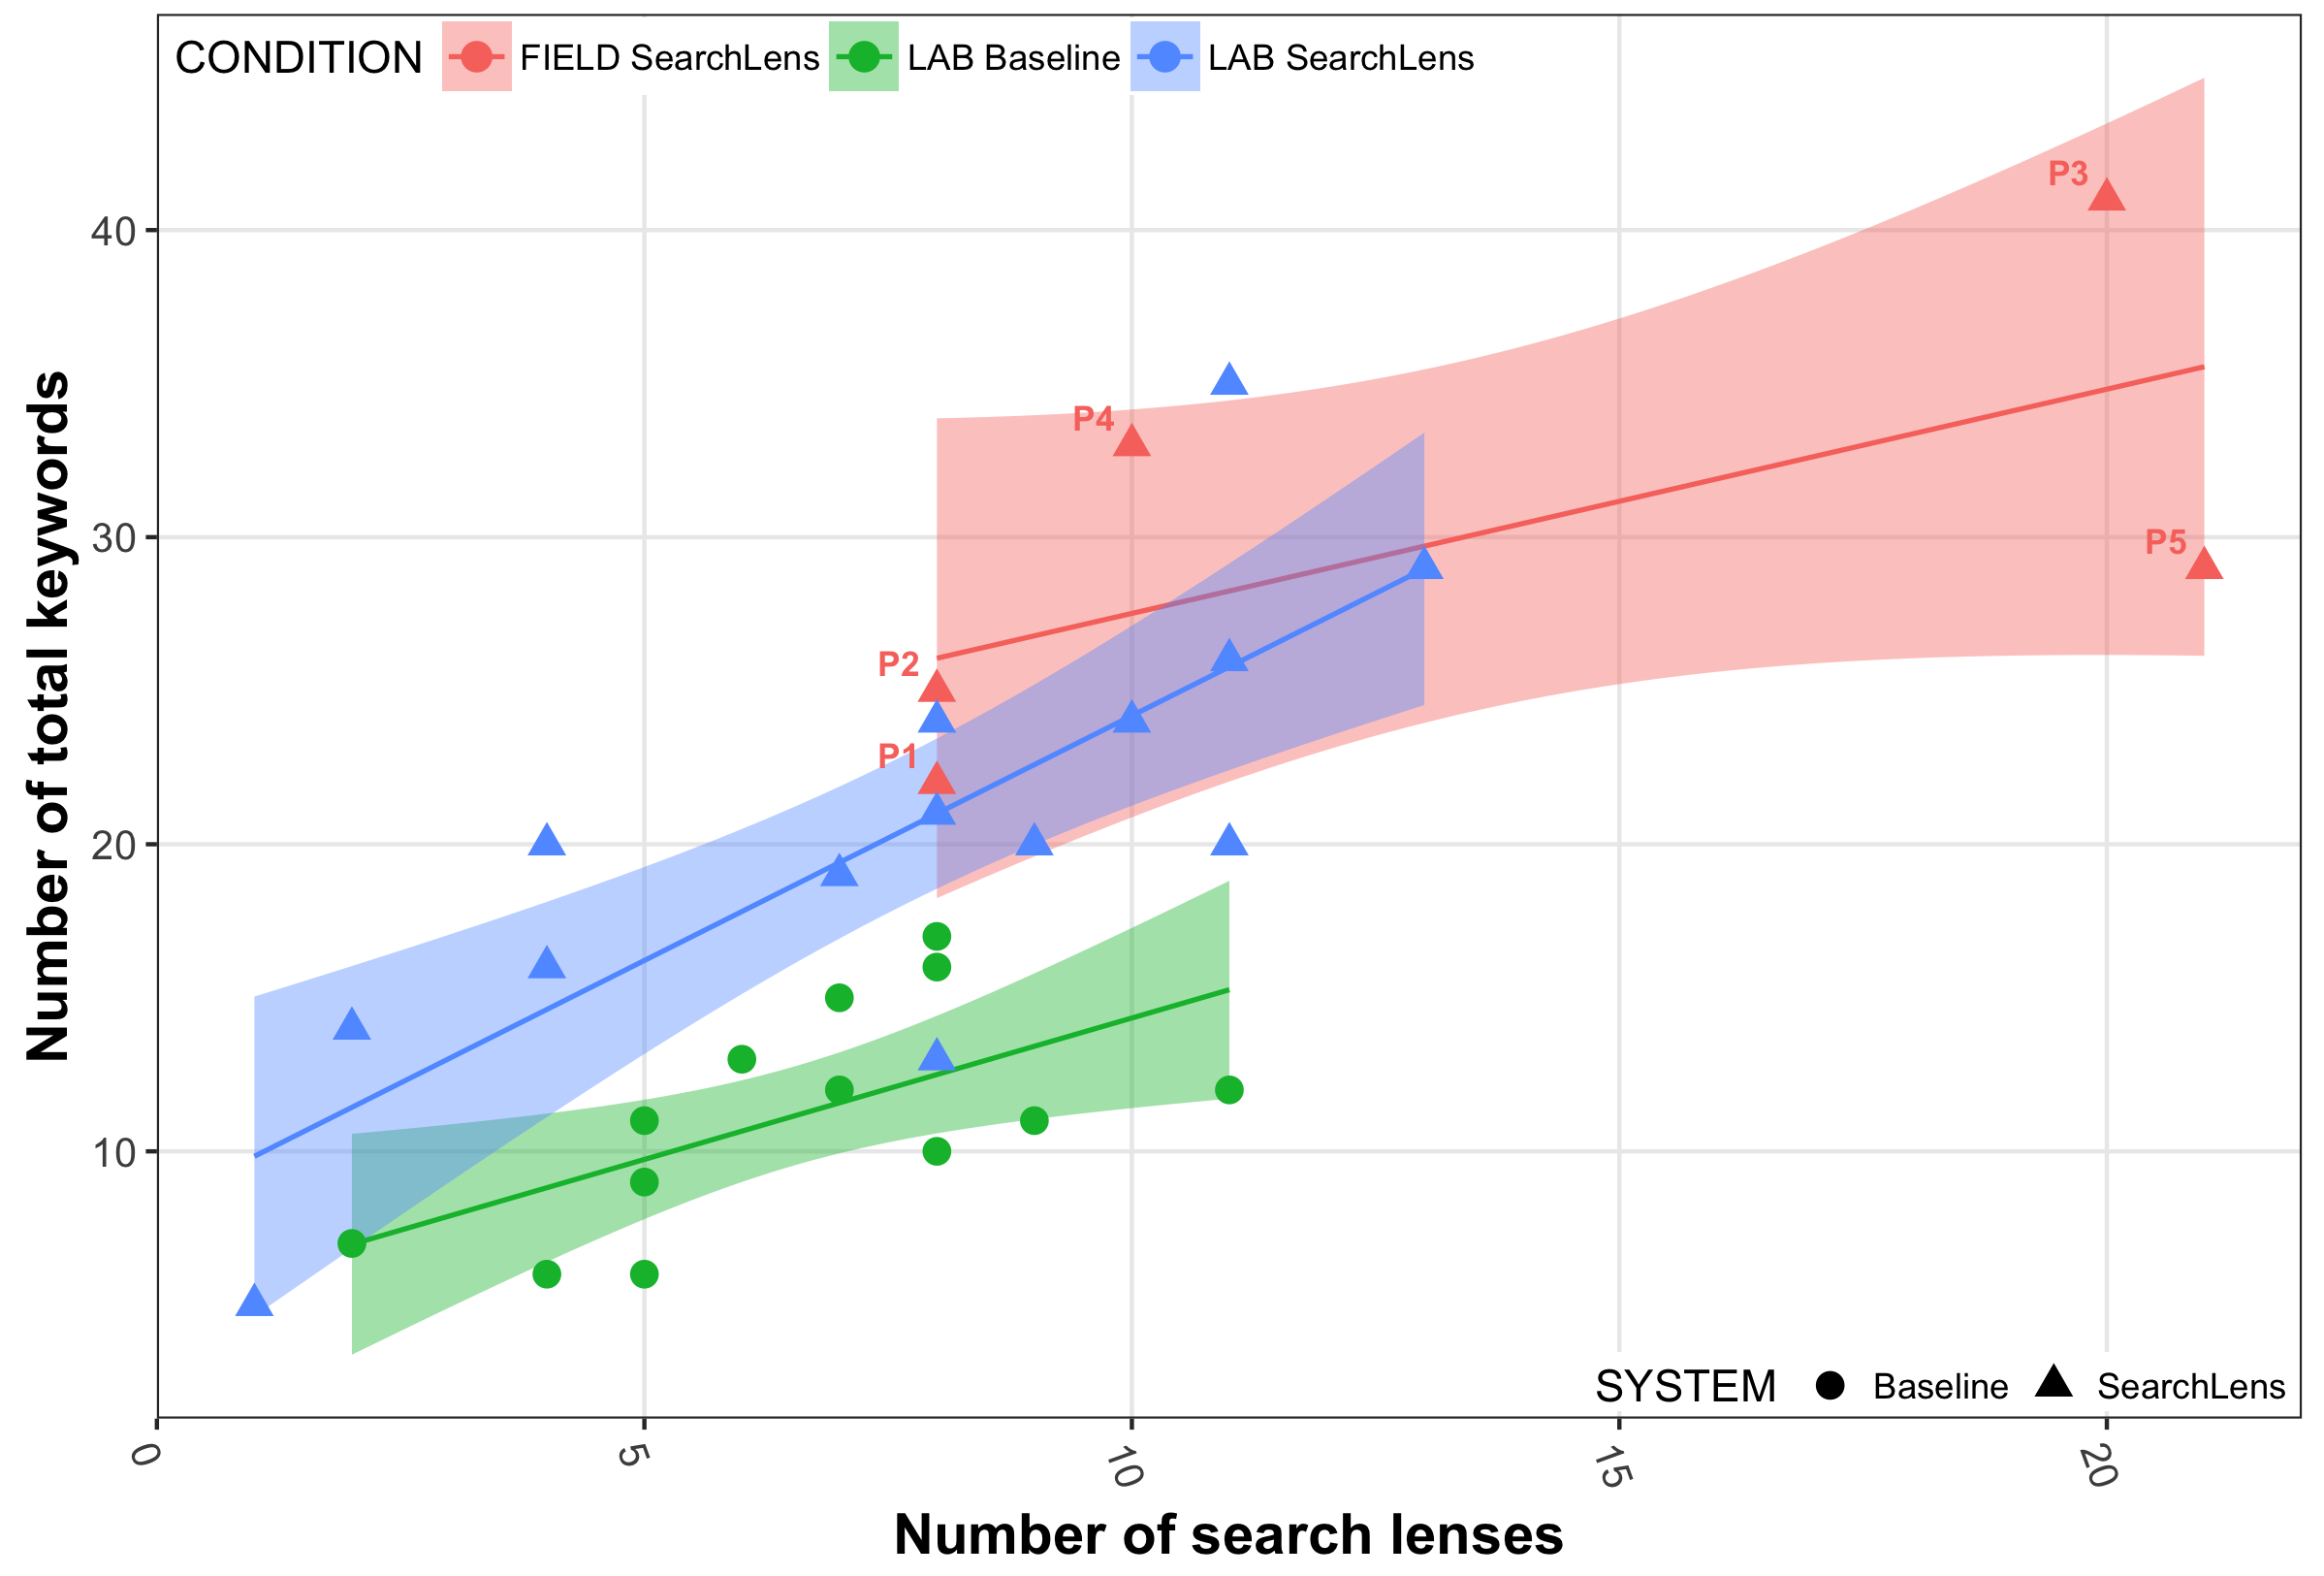
\includegraphics[width=0.8\columnwidth]{Chapters/SearchLens/figures/LensKeywordsCount.png}
    \caption[Number of Lenses and keywords under different conditions.]{Number of Lenses and keywords specified by participants under different conditions. In the lab study with predefined search tasks, participants using SearchLens (blue) created a similar number of Lenses but used more keywords than the baseline condition (green). Participants in the field study (red) conducted their own tasks.}
    \label{fig:sl_counts}
\end{figure} 


%\subsubsection{Participants and Use Cases}

Participants created more Lens keywords when conducting their own tasks comparing to participants in the lab study (Figure~\ref{fig:sl_counts}). On average, participants in the field study created 13.40 (SD=3.65) Lenses, significantly more than participants in the lab study that created 7.64 Lenses (SD=6.54; t(17)=2.46, p<0.05). They also saved significantly more keywords than participants in the lab study (lab: 20.4, field: 30.0, t(17)=2.50, p<0.05).
Admittedly, it can be difficult to measure how much time participants actually spent using SearchLens in the field, nevertheless, results suggest that participants were able to accumulate more interests Lenses over a three day period than participants who spent 60 minutes in the lab study.

All five participants conducted multiple tasks during the study. Many explored different types of restaurants that they liked in the city using multiple Lenses, using SearchLens to build \emph{``an overview interface for restaurants in the city that I might like''} (P1, P3, P4, P5). Participants also had more specific goals, including to check if there are vegan restaurants she has not discovered yet (P5), restaurants that serve bubble tea (P2), pizza places that offer Chicago deep dish-styled pizza (P3), and Mexican restaurants that has vegan options on the menu (P2).

%Below is an overview of the tasks conducted by the five participants. The number of Lenses and keywords saved by each participant is shown in Figure~\ref{fig:sl_counts}. In the next subsections, we list common use cases and strategies as reported by the participants in the interviews and post-survey:


%\begin{itemize}

%\setlength\itemsep{-2pt}
%    
%    \item \textbf{P1} conducted multiple tasks to explore different types of restaurants in the city.
%    \item \textbf{P2} used SearchLens to find Mexican restaurants with vegan options as well as places that have bubble tea.
%    \item \textbf{P3} used SearchLens to search for pizza places that offer Chicago deep dish-styled pizza, and as well as to explore the different options in the city.
%    \item \textbf{P4} was similar to P1.
%    \item \textbf{P5} was similar to P1, but specifically looked for vegan restaurants she had not yet discovered.
%\end{itemize}

%Participants P1 through P4 lived in the city for the past 3-4 years, while P5 is new to the city.

%\subsubsection{Behavior Logging}

%We recorded the behavior of our participants while using the SearchLens interface. Figure~\ref{fig:sl_counts} shows the number of Lenses and keywords each participants under different conditions collected during the study, and Figure~\ref{fig:behavior} and~\ref{fig:lens_behavior} shows the number of action participants performed under different conditions.  In general, participants in the Field Study conducting their own tasks generated more Lenses and keywords, and also performed operation on refining their Lenses. However, they were performing different search tasks and spending more time on the system than participants in the Lab Study.



\subsubsection{Refining Lenses}

While participants reported creating Lenses based primarily on prior knowledge, all five participants also reported refining their Lenses throughout the process. Several cited that the shaded cells of the visual explanation helped them quickly noticed some keywords were too uncommon, and that an important concept of interest was missing from the search results (P1, P2, P5). One also mentioned noticing and removing ambiguous keywords when using the mention filtering features (P4). Participants also learned about new keywords which they added to their Lenses, sometimes replacing existing keywords, from both the suggestions (P1, P2, P3, P5) and from the reviews (P1, P2). Interestingly, the behavioral logs (Table~\ref{tab:actions}) suggest they frequently discovered them from the systems' suggestions, indicating the value of the word2vec approach which we initially were concerned about for being noisy. This also points to potential future work in auto-suggesting Lenses which we intentionally avoided here due to concerns about agency and explainability. 

\subsubsection{Breadth and Depth}

Participants created both general, breadth-oriented Lenses and more specific, depth-oriented Lenses. P4 specifically mentioned that it was useful being able to search for different genre (i.e., American, Mexican, or Indian restaurants) and at the same time pay attention to very specific dishes (i.e., cheese steak sandwich made with chicken), while still being able to see how each result match with different things, citing that ``\emph{more specific things are hard to search for on Yelp.}'' Alternatively, P3 presented an interesting use case for deeper exploration of a specific genre, by first creating an more general Indian Food Lens, and then creating multiple more specific Lenses describing specific dishes from different regions of India, generating an overview of different styles of Indian restaurants in the city. This suggests that some users may want to create higher level groups of Lenses

\subsubsection{Reusing Lenses: Combinations and Task Resumption}

Participants reported their strategies for how they reused their Lenses, which can be broken down into two non-exclusive categories. The first use case we observed was task resumption between multiple search sessions (P1, P3, P4). Participants described having the ability to switch to a different sets of Lenses yet still keep the original Lenses for the future being useful (P3). One participant (P1) searched with a single Lens most of the time, but still cited that being able to re-enable Lenses from past sessions and to continue work on previous tasks and refined restaurants being useful. For the second use case, participants mentioned reusing Lenses in combination with other Lenses (P2, P3, P5). When asked about which of their Lenses were used in combination with different other Lenses, participants reported Lenses that concerned style and environment (\emph{Cute and Quirky} (P5), \emph{Atmosphere and Vibe} (P2, P5), \emph{Friendly Staff} (P3)), price (\emph{Inexpensive} (P2, P3), \emph{Large Portion} (P3)), and some food-related but not for a general genre (\emph{Fresh} (P2), \emph{Fast Casual} (P2), \emph{Vegan Options} (P2, P5), \emph{Strong Beer} (P3)).

\subsection{Overall Usefulness and Other Usecases}


Through the lab and the field studies, we found evidence that using user-generated Lenses to provide visual explanation for deeper exploration was beneficial and effective in incentivizing users to externalize and iteratively refine their interests using Lenses. This occurred throughout the search process almost twice as frequently when compared to participants in the baseline condition which did not include the visual explanation and exploration features (Figure~\ref{fig:sl_baseline}). As a result, participants using SearchLens created richer Lenses with nearly double the number of keywords on average compared to participants in the baseline condition. Participants also frequently used the visual explanation feature to explore the individual items in their search results, filtering reviews using different keywords in their Lenses 25.9 times on average. To test SearchLens in real-world settings, participants in the field study conducted their own tasks, and provided insights into their strategies in building and refining Lenses, as well as their strategies of composing and reusing Lenses across context and across search sessions over a three day period.

From the field study interviews, three out of the five participants said that they actually found and saved interesting restaurants during the study, and intend to visit those restaurant in the near future (P1, P3, P4). P1 in particular went to one of the restaurants he discovered using SearchLens and was happy about the visit, and P3 used SearchLens to complete a previous task, saying ``\emph{I wanted to try deep dish pizza for some time since I moved to US. Finally found one near the city. Kudos!}'' All participant expressed that they would be interested in using SearchLens in the future if available, many also cited other scenario that might benefit from SearchLens. P2 pointed to scenarios where he needed to ``\emph{find a place for many people that may want different things}'', and mentioned that SearchLens would be useful when her family visits her soon for his graduation. These results suggest that SearchLens was effective at helping users effectively find items that matched their specific interests. 

\section{Discussion and Limitations}

One limitation of the current implementation of SearchLens is its lack of ability to filter restaurants using their metadata, such as geographic location. We intentionally did not expose this information to our participants so we can focus our studies on allowing them to build personalized Lenses. However, practical systems would likely combine both paradigms to maximize efficiency. Utilizing metadata can also augment user-defined Lenses, for example, taking into account whether the a review that matched a specific Lens was positive or negative and whether the review poster's interests matched with the user's personal interests. However, the interactions between the two paradigms would require further studies. On the other hand, utilizing existing techniques for query term generalization beyond stemming or lemmatization, such as synonyms, semantic word models, or query expansion, can potentially improve recall, but their effects on the visual explanations would also require further studies.

Another obvious limitation of SearchLens it that it required more user effort upfront in order to receive the benefits provided by the system, such as reuse, explanation, and exploration. On a 7-point Likert scale, most participants from our lab study responded favorably in the post-survey to this trade-off with 64\% agreed or strongly agreed that SearchLens is an improvement to the traditional search interfaces, and another 21\% somewhat agreed with the statement, however, the long-term effect remained to be seen. One way to extend SearchLens is to combine machine learning and information retrieval approaches to reduce the effort of building Lenses, such as building interest profiles automatically, or using collaborative filtering and query expansion for expanding or inferring Lenses automatically \cite{ahn2007open,sarwar2001item,xu1996query}, or word-sense disambiguation techniques for resolving ambiguous keywords \cite{yarowsky1995unsupervised}.

Alternatively, we could also explore ways to allow users to share their Lenses with each other through explicit or implicit collaborations. For example, one participant mentioned ``\emph{It would be nice if I can see what Lenses a local person would use if I'm traveling, because I always try to ask the locals about where I should eat.}'' Allowing access to Lenses created by previous users or expert users could potentially enable expertise transfer and accumulation through continuing refinement of a set of Lenses. For example, locals and past travelers could iteratively curate a set of Lenses that leads to an interactive and explorable list of local specialties for future travelers.

Another promising direction is to more deeply explore the idea of user-generated interest profiles and how they could dynamically influence the different interfaces accessible to the user or interacting with users in more proactive ways.
Since we asked the field study participants to use SearchLens for their own tasks, most participants searched for restaurants in the city they lived in. Some participants that conducted more targeted search tasks (P2, P3, P5) mentioned that they were already familiar with most of the options in the city that fits their goals, but would still occasionally search online to see if there were new restaurants that match their interests (P2, P5).
As users continue to use SearchLens, the system will accumulate more understanding of what the users is interested in, and can potentially detect and notify the users of new information that might be of interests with high accuracy \cite{yang2006retroactive}.
Alternatively, existing users may use their repository of Lenses to explore or curate the restaurants in an unfamiliar city. Participants in the field study also pointed to the potential of Lenses being useful for other types of information and domain, including shopping (P2, P3), trip planning (P2, P5), buying a house (P2), and job hunting (P4). 


In this chapter we introduced SearchLens, a novel approach that allows users to specify and maintain their profile of multifarious and idiosyncratic interests. This enabled them to reuse and re-compose their different interests across scenarios, as well as maintaining context across multiple search sessions. To encourage users to put in the up-front effort of curating Lenses, we explored ways of using Lenses to provide immediate benefits of visual explanation and deeper exploration of search results. Across a lab and field study we observed that participants expressed their interests with significantly more query terms, and found benefits in the SearchLens approach, including being able to transfer and reuse their Lenses across contexts, being able to interpret new information that reflects their own personal interests with transparency, and working at multiple levels of specificity and hierarchy.
More fundamentally, being able to visualize and explore new information in ways that promote transparency can potentially empower users to be more aware of their online information diet. For example, as a way to manipulate their own social media feeds, and being more aware of how posts were selected or hidden. We believe SearchLens represents a first step towards a transparent and user-centered approach to addressing subjective and fragmented nature of information today.


%\section{Acknowledgments}

%This work was supported by the National Science Foundation (grants PFI-1701005 and SHF-1814826), Google, and the Carnegie Mellon University Center for Knowledge Acceleration.
